\documentclass[conference]{IEEEtran}
%\documentclass[conference]{acm_proc_article-sp}
\usepackage{cite}
%\usepackage{mathptmx}
\usepackage{graphicx}
\usepackage{myart,times}
% \usepackage{stfloats}
\usepackage{listings}
\let\labelindent\relax
\usepackage{enumitem} 
\usepackage{fancyvrb}
% \usepackage{framed}
% \usepackage{caption}
\usepackage{subcaption}
% \usepackage{subfigure}
%\usepackage{amsthm}
\usepackage[]{algorithm2e}
\usepackage{todonotes}
\presetkeys{todonotes}{inline}{}
\newcommand{\done}[2]{\todo[color=green!40]{#1\bf{#2}}}


% \usepackage[listings,skins]{tcolorbox}
\hyphenation{op-tical net-works semi-conduc-tor}
\newtheorem{definition}{Definition}
\newcommand{\titlea}{Static Detection and Automatic Exploitation of Intent Message Vulnerabilities in Android Applications}
\newcommand{\titleb}{Analysis of Android Applications for Intent Message Vulnerabilities}
\newcommand{\titlec}{Android Message Passing Analysis}
\newcommand{\titled}{Practical Exploit Generation for Intent Message Vulnerabilities in Android}
\begin{document}
\title{\titlea}


\author{
\IEEEauthorblockN{Daniele Gallingani}
\IEEEauthorblockA{University of Illinois at Chicago\\
Chicago, IL\\
Politecnico di Milano\\
Milano, Italy\\
Email: dgalli3@uic.edu}
\and
\IEEEauthorblockN{Rigel Gjomemo, V.N. Venkatakrishnan}
\IEEEauthorblockA{University of Illinois at Chicago\\
Chicago, IL\\
Email: \{rgjome1,venkat\}@uic.edu}
\and
\IEEEauthorblockN{Stefano Zanero}
\IEEEauthorblockA{Politecnico di Milano\\
Milano, Italy\\
Email: stefano.zanero@polimi.it}
}

%\numberofauthors{4}
%\author{
%\alignauthor
%Daniele Gallingani\\
%       \affaddr{University of Illinois at Chicago}\\
%       \affaddr{Chicago, IL}\\
%       \affaddr{Politecnico di Milano}\\
%       \affaddr{Milano, Italy}\\
%       \email{dgalli3@uic.edu}\\
%       \email{daniele.gallingani@mail.polimi.it}
%\alignauthor
%Rigel Gjomemo\\
%       \affaddr{University of Illinois at Chicago}\\
%       \affaddr{Chicago, IL}\\
%       \email{rgjome1@uic.edu}
%\alignauthor
%V.N. Venkatakrishnan\\
%       \affaddr{University of Illinois at Chicago}\\
%       \affaddr{Chicago, IL}\\
%       \email{venkat@uic.edu}
%\alignauthor
%\and
%Stefano Zanero\\
%       \affaddr{Politecnico di Milano}\\
%       \affaddr{Milano, Italy}\\
%       \email{stefano.zanero@polimi.it}
%}

% \author{
% \IEEEauthorblockN{
% Daniele Gallingani\IEEEauthorrefmark{1},
% Rigel Gjomemo\IEEEauthorrefmark{2},
% V.N. Venkatakrishnan\IEEEauthorrefmark{3} and
% Stefano Zanero\IEEEauthorrefmark{4}
% }
% \IEEEauthorblockA{\IEEEauthorrefmark{1}University of Illinois at Chicago\\
% Chicago, IL\\
% Politecnico di Milano\\
% Milano, Italy\\
% Email: dgalli3@uic.edu}
% \IEEEauthorblockA{\IEEEauthorrefmark{2}University of Illinois at Chicago\\
% Chicago, IL\\
% Email: rgjome1@uic.edu}
% \IEEEauthorblockA{\IEEEauthorrefmark{3}University of Illinois at Chicago\\
% Chicago, IL\\
% Email: venkat@uic.edu}
% \IEEEauthorblockA{\IEEEauthorrefmark{4}Politecnico di Milano\\
% Milano, Italy\\
% Email: stefano.zanero@polimi.it}
% }

\maketitle


\begin{abstract}
Android's Inter-Component Communication (ICC) mechanism strongly relies
on  Intent messages. Unfortunately, due to the lack of message
origin verification in Intents, implementing security policies based
on message sources is hard in practice, and completely relies on the
programmer's skill and attention. In this paper, we present a framework for automatically detecting Intent input validation vulnerabilities. We are thus able to highlight component fragments
that expose vulnerable resources to possible malicious message senders. Most importantly, we advance the state of the art by developing a method to automatically demonstrate whether the identified vulnerabilities can be exploited or not, adopting a formal approach to automatically produce malicious payloads that can trigger dangerous behavior in vulnerable applications. We therefore eliminate the high rate of false positives common in previously applied methods. We test our methods on a representative sample of applications, and we find that 29 out of 64 tested applications are detected as potentially vulnerable, while 26 out of 29 can be automatically proven to be exploitable. Our experiments demonstrate the lack of exhaustive sanity checks when receiving messages from unknown sources, and stress the underestimation of this problem in real world application development. 
\end{abstract}


%\IEEEpeerreviewmaketitle

% !TEX root =  ../main.tex
\section{Introduction}

% Out of a 6.8 billion alleged mobile phone subscribers~\cite{ict-facts-2013},
% the Android platform enjoys a 75\% market share, according to the most recent
% surveys~\cite{gartner-stats-2013,idc-android-2013}.
% % Along with the
% % number of Android devices, the size of the official app market,
% % the Google Play Store, is astonishing: it reportedly totaled
% % 25 billion downloads in September~2012~\cite{apps25bil}, and it
% % is foreseen to pass the threshold of 1 million available
% % applications~\cite{apps1m}.
% Unsurprisingly, Android is quickly becoming the target of choice for
% cybercriminals~\cite{trendmicro-q3-2012}. While currently the
% most prevalent threat consists of malicious apps, according to McAfee's most
% recent report~\cite{mcafee-q1-2013}, spyware and targeted attacks
% are gaining hold. Therefore, vulnerabilities at the application
% level will soon become an important target for attackers.

Android applications are formed by logically separated
components that communicate with each other through two message passing mechanisms:
\emph{Binder} and \emph{Intents}. \emph{Binder} is a lightweight remote procedure call
mechanism, mainly used in service-to-service communication, while
\emph{Intents} are the most used inter-component and inter-application communication mechanism.
\emph{Intents} are used for data exchange, as well as for requesting the
execution of a procedure to another application.

Unfortunately, the Android Intent Passing mechanism does not provide the
receiving component with any information concerning the origin of an intent.
This facilitates the creation of spoofed intents with malicious input data. If such
malicious input is not properly validated or sanitized by an application
before being processed, it may subvert its state and control flow in unexpected
ways. This attack vector may lead to a wide range of attacks, not only against
the application itself, but also against other applications that receive and
process data from the vulnerable app. %In practice, implementing an application
%component that safely processes input messages is hard.

%The only practical filtering mechanism is an all-or-nothing scheme, where components either
%disallow any Intent coming from a different process, or accept any Intent matching a signature.
%Signatures for all the components are declared in the application manifest file, easily accessible
%to any potential attacker.

%This creates an important class of vulnerabilities, in which a malicious application
%could target another (vulnerable) application to compromise its internal state, or to
%perform through it actions on remote resources bound to it.

% via \emph{intent-filters} on the official Android documentation web site.
Previous research works studied applications and the Android ecosystem to
identify components that are exposed to receiving intents from untrusted
applications \cite{chin2011analyzing}. Others studied how applications can
circumvent Android's permission checking by delegating execution of operations
to applications with elevated permissions \cite{felt2011permission}. 
\cite{Grace:Android:2012} analyzed permission leaks in Android apps in order to identify permission leakage. 
Finally, CHEX~\cite{Lu:CHEX:2012} develop static analysis techniques to
check whether there exist dataflows that could lead to component hijacking vulnerabilities. 

% Yet other work provides a language
% for
% specifying and proving the safety of unknown applications \cite{LanguageBasedSecurity}.

However, a common shortcoming of prior literature is not being able to automatically verify 
the \emph{practical exploitability} of component hijacking vulnerabilities. For instance, 
CHEX~\cite{Lu:CHEX:2012} identifies 254 apps with suspicious data flows. A subsequent manual 
analysis by the authors, however, identified that 48 out of these 254 apps were false positives. 
Such false positives are due to two main reasons:
% \setlist[itemize]{noitemsep, topsep=10pt}
\begin{itemize}
\item {\em Precision issues in static analysis}. Static analysis techniques approximate the behavior of programs. Usually, a sound approximation is sought, by including all possible behaviors. However, to do so, approximations err on the side of excess, including additional behaviors that are not really present, such as dead code (i.e. paths that are never feasibly exercised). Since such additional paths are considered during dataflow analysis, they may lead to false instances of suspicious dataflows.  

\item {\em Effect of security-critical actions of code}. Analysis techniques in state-of-the-art approaches to this problem only take into account the existence of potential suspicious paths. They ignore, however, the effect of the code along those paths, such as the use of input validation to mitigate intent spoofing vulnerabilities~\cite{chin2011analyzing}. Since such techniques can effectively obviate the security issues, ignoring their effectiveness leads to a large number of false alerts.
\end{itemize}

In this paper, we improve the state-of-art by automatically developing proof-of-concept exploits against applications, to effectively prove that they are vulnerable to intent message vulnerabilities. Developing proof-of-concept exploits helps minimize the risk of false alarms, and thus it increases the usability of the approach. 

To do so, we statically analyze the application to identify data-flows under an attacker's (indirect) control. We design an analyzer that is able to follow such flows and identify Intent data that may affect either directly or indirectly the
results that a component produces and sends in output. We formulate the problem as
an Interprocedural Distributive Environment
one, which allows us to efficiently deal with inter-procedural flows. Once such suspicious flows are identified, we develop techniques to analyze the operations (e.g., sanitization) along the identified flows. At this point, we use a constraint solver to develop concrete proof-of-concept exploits, thereby confirming the presence of the vulnerability. Finally, we are able to demonstrate the vulnerability by developing an {\em attacker app}, capable of launching these exploits on actual applications. It is important to note that, similarly to~\cite{Lu:CHEX:2012}, our approach works on unmodified Android apps, without requiring any special information, nor access to the source code.

We test our approach on 64 popular applications from the Google Play store. Of these, 29 exhibit potential vulnerabilities, and for 26 of these, we
are able to automatically generate an exploit, i.e. spoofed intents that trigger and demonstrate those vulnerabilities. 
We discuss in depth the results of this evaluation and analyze manually the applications to confirm them.
We can thus confirm that many popular applications do not implement appropriate security countermeasures for Intent communications. Indeed, from our
analysis we observed that most applications only check if malformed Intent payload tuples are received, but such checks are meant to avoid errors, and are
thus far from sufficient to stop a determined attacker.

In summary, we make the following novel contributions:
\begin{itemize}
% \item we study in depth the attack surface and the impact of vulnerabilities in
% apps related to Intent message passing.
 \item We provide a static analysis method to automatically detect data flows that potentially allow
 Intent data to affect the results sent in output by the applications, i.e. to identify potential vulnerabilities (Sections \ref{sec:problem}, \ref{sec:approach}). 
 \item We provide a sound formulation of this problem as an Interprocedural Distributive Environment problem(Section \ref{sec:implementation}).
 \item We describe an approach to automatically generate Intent examples that trigger a malicious behavior, thus automatically validating the discovered vulnerabilities (Section \ref{sec:implementation}).
 \item We develop an {\em attacker app}, that is capable of delivering malicious exploit inputs to exercise these vulnerabilities (Section \ref{sec:implementation}). 
\end{itemize}

We report our evaluation results in Section \ref{sec:results}. In Section \ref{sec:related} we review  related works. Finally, in Section \ref{sec:concl} we draw our conclusions.


% !TEX root =  ../main.tex
\section{Problem Statement}
\label{sec:problem}

%In the following, we will analyze the class of vulnerabilities that arise from the
%lack of controls on messagge passing through Intents, and we will formalize the problem we want to solve.

In this section, we provide a running example and illustrate the problem we are exploring.

% \subsection{Android Communication System Overview}

% Android applications are formed by a set of logically separated components
% (Activities, Services, Broadcast Receivers) that can communicate with each other
% during execution. Communication among these components is carried out by the IPC
% service of the operating system through a message passing mechanism, based on
% \emph{intents}. Essentially, \emph{intents} are messages containing a data portion, an action portion
% that tells the receiving application how to process the data, a category, and an optional
% component portion, which designates the receiving component.

% Components belonging to the same application can always communicate among each other via intents.
% To be able to receive intents sent by external applications, a component must
% explicitly declare an \emph{intent-filter} in the application's manifest file.
% Intent-filters describe the structure of intents (data types, actions, etc) a component is
% willing to receive and process. The operating system uses these \emph{intent-filters} to
% identify the recipient component of an intent, if not explicitly stated.

% The ability to receive intents from external applications is an important design feature of Android.
% In this way, applications can delegate tasks and communicate.
% The intent passing mechanism represents an often trusted communication channel
% in Android. However, Android itself does not provide mechanisms for applications
% components to verify the origin of intents. In particular, the most vulnerable
% components are those that expose intent-filters in the manifest file, enabling any application
% to send messages to those components. 

% \subsection{Threat Model and Running Example}
\textbf{Threat Model}. In our threat model, an attacker first analyzes the manifest file to identify exposed components that can receive intent messages. An example of such a component is depicted in Listing \ref{lst:example}, where the \textit{onCreate} method (line 1) is called to start a component. Next, the attacker identifies statements inside those components whose execution may be subverted to the attacker' s advantage. These statements may include network operations, database operations, updates to GUI elements and so on, and their execution may be subverted by modifying their parameter values, e.g., URL-s where data are sent by network operations, database queries, and the text of GUI elements. One such statement, dealing with a network operation is the HttpPost object creation in line 19. If the attacker is able to modify the value of the \textit{url} variable to a domain under the attacker's control or the value of the \textit{httpPar} variable to a string containing a cross-site scripting attack, then the component can be used to leak data to the attacker's web site or to execute a cross-site scripting attack, respectively. Another statement that may be of interest to an attacker is the one on line 31, which sets the path of a file that is ultimately sent over the network. If the attacker is able to modify the value of the variable \textit{p} (for instance, by including ``..'' in the path to perform directory traversal) together with the variable \textit{url}, then the component can be used to send arbitrary files to a host under the attacker's control. 
%We note however, that lines 13-14 sanitize the value of the \textit{file} variable before it reaches line 32. 
In the rest of this paper, we call such statements targeted by an attacker \textit{sink} statements.

Under this threat model, the only way in which the attacker can try to modify the parameters of the sink statements is by sending a specially crafted intent to the component via a malicious application installed on the user's phone. Thus, if the component is exposed, the attacker can control the values that that component receives in input (e.g., lines 2-5).

This attack vector has been recognized in the past by researchers and developers alike~\cite{Lu:CHEX:2012,chin2011analyzing,AppIntent,IntentsForDevelopers}. Two recommended practices for limiting this type of attacks are to not expose components needlessly and to sanitize and validate the data in input to the components. However, as often happens in application development, secure coding practices are not always followed. In fact, as shown by two independent studies of the first practice, a large percentage of applications still exposes components needlessly~\cite{Epicc,chin2011analyzing}. In addition, as shown by other studies, there may exist execution paths from (exposed) source statements to sensitive sinks~\cite{Lu:CHEX:2012}, along which data may flow. However, the presence of a path does not necessarily imply that an attack is feasible. In particular, applications may perform several operations along that path, such as sanitizations and other business logic operations. 

% \renewcommand{\lstlistingname}{}
\begin{lstlisting}[caption={Source code of a vulnerable application},label={lst:example},numbers=left,xleftmargin=1cm,basicstyle=\ttfamily\scriptsize ]
void onCreate(Bundle savedInstance) {
 Intent intent=getIntent();
 String host = intent.getStringExtra("hostname");
 String user = intent.getStringExtra("username");
 String file = intent.getStringExtra("filename");
 String url="http://www.example.com";
 if (host.contains("example.com"))
   url = "http://" + host + "/";
 if (file.contains(".."))
   file = file.replace("..", "");
 String userId = getUserID(user);
 if (userId != -1)
   textView.setText(user_name);
 String b64File = toBase64(file);
 String httpPar = toHttpParams(b64File,user_id);
 . . .
 try {
   DefaultHttpClient httpC = new DefaultHttpClient();
   HttpPost post = new HttpPost(url+httPar);
   . . .
   httpC.execute(post);
 }
 catch(IOException e) {
   e.printStackTrace();
 }
}
String toBase64(String p) {
 if(p=null || p.equals(""))
   p = "/data/data/com.example/defaultFile.pdf";
 else
   p = "/data/data/com.example/public/" + p;
 byte[] bytes = InputStream.read(p);
 String b = Base64Encoder.toString(bytes);
 return b;
}
\end{lstlisting}
% \normalsize
% \caption{Source code for the vulnerable application\label{fig:example-code}}
% \end{subfigure}
% \vspace{0.15in}
% \caption{A vulnerable application and its implementing code.}

In our example, we delineate three different operations that deal with the input variables. The first operation is a sanitization (lines 7-8) of the variable $host$. This sanitization is not sufficient, since an attacker can use any host name that contains the ``example.com'' string, e.g., ``malicious.example.com'' or ``example.com.com''. The value of \textit{host} set by the attacker inside the intent therefore flows unmodified to the sink statement at line 19. The second operation is also a sanitization (lines 9-10), which removes eventual ``..'' substrings from the file name to prevent directory traversal attacks. This sanitized value is then used later in line 31, which also adds a predefined prefix to the path. Thus, even though an attacker may be able to control to a certain degree the value of the variable \textit{p} at the sink statement (line 32), he cannot use it to perform a directory traversal attack. The third operation (lines 11-13) checks that the \textit{user} exists and sets a GUI element to a default user name if it does not exist. After this point, the value of the variable \textit{user} is not used by the program anymore. 

As has been recognized by previous work, to detect this type of vulnerabilities, it is important to correctly identify paths that starting from the \textit{source} statements enable an attacker to influence the variable values at the \textit{sink} statements. However, the existence of a path does not imply that an attack is feasible. To precisely identify exploit opportunities and prevent them, the operations performed on the variable values along that path must also be considered. In fact, these operations may include  sanitizations (e.g., lines 9-10), and other business logic operations (e.g., lines 11-13) that, while allowing an attacker to influence the values at the sink statements, make exploits unfeasible. An approach that includes these path operations in its analysis is therefore needed to precisely identify exploit opportunities and prevent them. Such an approach must also provide a vulnerability proof under the form of malicious input to the component, in order to verify the vulnerability. In the rest of the paper, we present a method for automatically detecting such vulnerabilities and providing proofs for them. 

%Rigel: this may be fitted for later
%The constraints for this variable will look like:
%\lstset{numbers=left, basicstyle=\ttfamily\scriptsize, breaklines=true}
%\begin{lstlisting}
%$hostname.contains("example.com") ->
%   $url :=  "http://" + $hostname + "/"
%(not $hostname.contains("example.com")) ->
%   $url :=  "http://www.example.com/"
%\end{lstlisting}

%Since the second clause does not lead to a propagation of $hostname$ to the sink, the solver is
%able to generate an exploit satisfying the first constraint. The solution will be $example.com@$ where the ``$@$'' symbol stays for any string.

%\item \emph{Exhaustive sanitization}. This happens for the path parameter encountering one control (line $13$) and two manipulations at line $14$ and $32$. Whereas the check and the first manipulation can be easily passed by providing a non-null string and not containing any ``$..$'' sequence, this is not sufficient for an attack to succeed. Indeed the string preponed to the path parameter at line $32$, binds the path to the application public folder. This manipulation and the
%absence of the double dot sequences in the path variable successfully prevents an attacker access of the application private files.
%Here below are the constraints:
%\lstset{numbers=left, basicstyle=\ttfamily\scriptsize, breaklines=true}
%\begin{lstlisting}
%$filename.contains("..") ->
%   $filename.replace("..", ".")
%$filename.length > 0
%$filename := "/data/data/com.example/public/" + $filename;
%\end{lstlisting}
%In this case, in order to have a correct problem formulation, we need to consider the sink semantic.
%The correct formulation for the $InputStream.read$ sink includes one more constraint for the string
%to be free (i.e. without manipulation).


%\item \emph{Unreachable sink}. Parameter $username$ is not exploitable.
%For this example we need to assume that the function $getUserID$ (line $10$) returns the user id
%if a username is found in the local database, $-1$ otherwise.
%A solution to this constraint can not be found since it would assume a complete knowledge of the
%dynamic environment, represented in this case by the local database.
%
%Also in this case the solver will be unable to find a solution for the constraint, since it will
%lack of bounds to produce a result. This vulnerability will be indeed reported correctly as unfeasible
%by our analyzer.


%\label{sec:running-example}
\todo{Edited code}
% \begin{figure*}[t]
% \centering
 %  \begin{subfigure}[b]{3.5in}
	% 	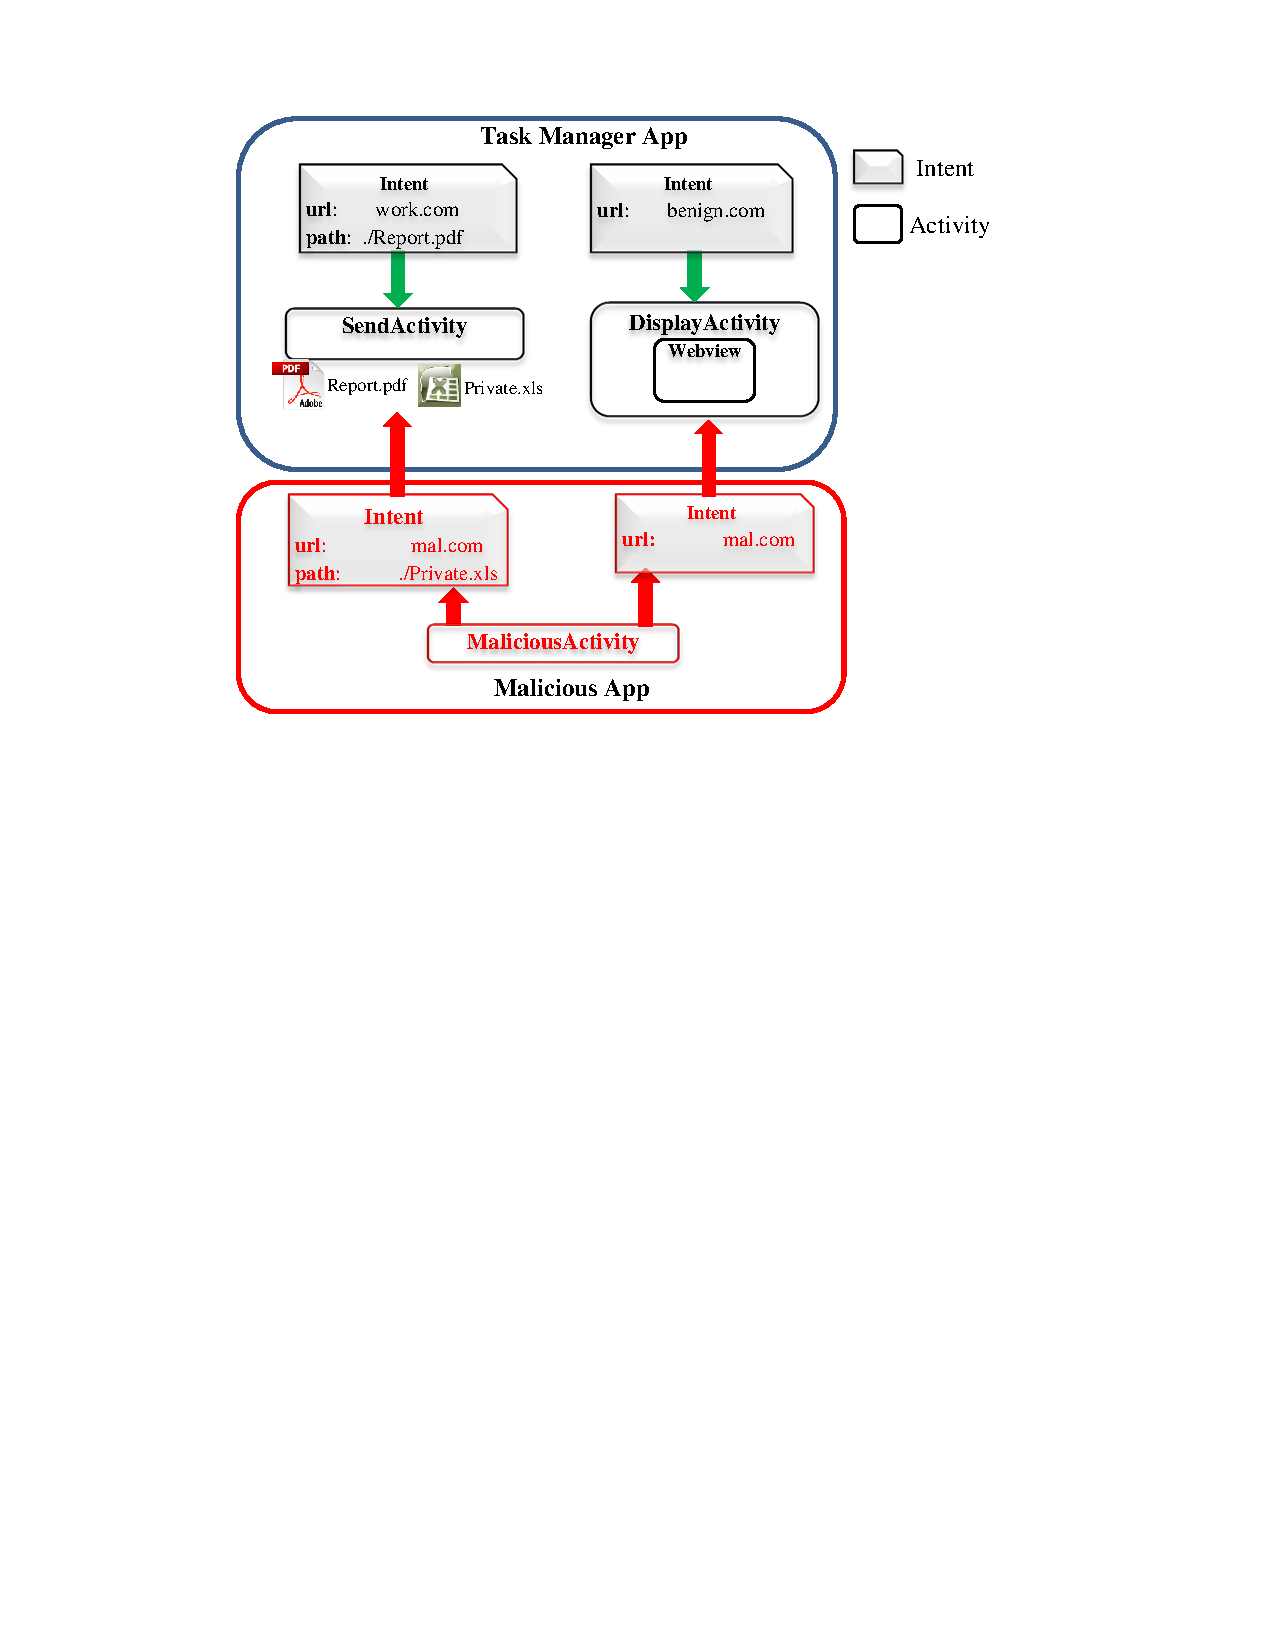
\includegraphics[width=3.3in]{./images/example.pdf}
 %                \caption{An example of vulnerable application.\label{fig:example-dia}}
	% \end{subfigure}%
        ~~~~~~~~~~~~ %add desired spacing between images, e. g. ~, \quad, \qquad, \hfill etc.
          %(or a blank line to force the subfigure onto a new line)
% \begin{subfigure}[b]{3in}
% \end{figure*}














%=========================
%TEXT FROM PREVIOUS VERSION


%We call this vector of attacks \emph{intent-spoofing attacks}. As illustrated by the examples,
%this attack may be performed by crafting intents that match the intent-filters declared by
%legitimate application components activities but contain data inserted by an attacker. The structure of such intents
%may be easily discovered by either looking at the manifest file of an application or by studying
%the (decompiled) code of the target application.

% \subsection{High Level Approach Overview}
% Our goal in this paper is to automatically identify opportunities for intent-spoofing attacks by modeling the relation between data input via intents and data output by an application component.

% Given an apk file, we first, we collect the entry points where malicious data may be received via intents and the sensitive operations
% where the results produced by a component are sent in output.
% %In this regard, we consider a wide range of operations executed
% %by framework method calls that includes output network operations, operations that execute SQL queries, and operations that update or create GUI elements. The range however may be extended to other output operations, such as those related to writing to the local file system.
% %For instance, lines 11 and 13 in the code example are identified as \emph{sources}, since
% %they are used to extract the data from the received intent.
% Next, using interprocedural data-flow analysis and taint analysis, we trace and collect the statements that process the intent data from the entry points to the sensitive operations that produce the output, thus obtaining several computation paths from the entry point to the output points. A detailed description of our analyzer is provided in Section \ref{staticAnalyzer}.
% %For instance, line 21 in the code example, which sends
% %data over the network is a \emph{sensitive sink} and the path comprising the statements at lines (11, 13, 14, 15, 18, 19, 21)
% %is a path where intent data flow from the sources to the sink.

% After the possible computation paths are identified, we need to prove that those paths are feasible at run time and that they can indeed be used by an attacker to subvert the intended behavior of the program.
% In fact, the existence of a path does not necessarily imply that the path can be useful for an attack.
% If, for instance, an activity validates the data along a path, then that path is not vulnerable. Our tool considers the different
% types of statements present in a path and automatically generates an intent with data that can be used to carry out an attack.
% This last step is described in more detail in Section \ref{sec:ExploitGenerator}.

%There are to ways to do this: fuzzying, app analysis.
%We are looking at analysis.
%High Level Overview:
%Goal: given the apk file, we want to
%see this app. During its execution it receives intent messages of two kinds.
%We want to see if an adversary can send from an untrusted component the integrity
%of an application. To understand, we must see how messages are received and processed
%by android. they are sent by a sender, received by a target,
%and processed in-application. Since the sender is untrusted we want ot
%identify in the app, the source. But this is not enough. Adversary needs to
%get to the sensitive sinks. In between we need to see how the message payload
%is processed.
%So our goal: Is a path possible between source and sink. This is data flow analysis:
%described in Section 3.2. Just identifying a path is not enough, we also need to prove that it
%is vulnerable. So we need to see what actions are being taken on that path.
%We need to


%
% Nonetheless, this type of open channel is present in many
%applications. Furthermore, due to the mistaken assumption that all intents sent at a target activity originate inside legitimate activities, the received data are not validated or sanitized before being passed to the rest of the application.
%Unfortunately, the Android IPC system does not provide mechanisms that can help verify the origin of an intent.


%\begin{itemize}
%  \item \textbf{Server attacks}: these attacks are similar to CSRF
%  attacks and to permission redelegation attacks identified in~\cite{felt2011permission}.
%  A malicious application sends to a component an Intent message that matches
%  the intent filters exposed by that component. Trusting that the intent originates
%  from a legitimate activity, the component does not validate the intent's data,
%  processes them according to some semantics and sends a request to a remote server.
%  Similarly to CSRF attacks, the request will be created within the normal request context.
%  That is, the request may be augmented with additional information, e.g. user-session
%  identifiers. The attack described in the example belongs to this category. %The attack, in this case, can be crafted
%%transparently with respect to client/server full-stack architecture, but taking
%%in consideration only Intent payload parts included in the request.
%
%%  As example, we can think of a bank application in which the mobile wire
%%transfer is implemented by the help of two activities: in the first activity,
%%the user is requested to insert the payee account and the amount. When the users
%%confirms, the information is sent as Intent payload to a second activity which
%%commits the transaction on the bank server. An attacker, by crafting the
%%exchanged Intent, could induce the second activity to perform a transfer on
%%behalf of the user to an arbitrary beneficiary.
%
%  \item \textbf{Storage attacks}: if intent data are used to
%build a query unsafely, even in case of Intent messages
%exchange we can have classical SQL Injection attacks \footnote{what does 'even in case of
%Intent messages exchange mean?}. Besides SQL Injection
%attacks, there can be identified other potentially dangerous attacks where the
%Intent receiver logic includes local storage operations and it is exposed via Intent
%receivers.
%%  These attack target logical vulnerabilities in application design, i.e.
%%situations in which local storage modifications are delegated to some particular
%%component which is queried via Intents.
%
% For instance, let's take into consideration another two activities example that implements a
%PIN change in an application where this code is used to guarantee
%application access. In the first activity a new PIN is collected from
%the user, then, in the second activity the old PIN is replaced with the new one
%by a database query. Similarly to the previous case, an attacker could arbitrary
%change the PIN by crafting an Intent with a different PIN, denying further application
%access to the user.
%
%  \item \textbf{Phishing attacks}: often intents are used to send data that
%  are displayed by the target Activity to the user.
%  An attacker could craft an intent containing fake data and send this intent to
%  the target Activity, thus prompting the fake data to the user.
%  To make this attack more effective, an attack may be designed to launch
%a series of Activities that exactly reconstruct the Activity sequence of
%the application, modifying the data displayed to the user at points of the
%attacker's choosing \footnote{we spoke about this type of attack before but the description
%must be more convincing. If we leave it at this rough level of detail it may sound
%unconvincing to the reader}.
%In this case, the deception could be very effective, since the
%user may think at herself as the author of the sequence of actions that produced
%the prompted screen.
%
%  A particular and remarkable variation of this attack is feasible when the intent
%  contains a URL of a page to be loaded in a web view. The vulnerable component
% In this case the attack
%can be even more effective, because of the image and general visual context
%that can be recreated inside a web view \footnote{is it more effective because
%it is easier to craft a web page very nicely?}.
%\end{itemize}
%
%This attack channel has been recognized by
%Android developers and researchers alike \cite{chin2011analyzing,felt2011permission}.
%In addition, application developers are warned against exposing activities via \emph{intent-filters} on
%the official Android documentation web site. Nonetheless, this type of open channel is present in many
%applications. Furthermore, due to the mistaken assumption that all intents sent at a target activity originate inside legitimate activities, the received data are not validated or sanitized before being passed to the rest of the application.
%Unfortunately, the Android IPC system does not provide mechanisms that can help verify the origin of an intent.
%
%An important thing to note at this point is that just the presence of an open channel does not
%necessarily imply that sensitive operations will be carried out by sending a spoofed intent.
%In fact, an open channel is exploitable in meaningful ways only if the
%flow and use of intent data inside an activity leads to eventually sensitive
%operations such as sending files to email addresses.
%
%The problem that we deal with in this paper is to automatically find \emph{sensitive paths} from the
%points in which intents are received (\emph{sources}) to sensitive API operations (\emph{sinks}) inside an
%application component.
%We use a rather general definition of sensitive API operations, which includes network communication
%APIs, database APIs, and UI APIs. This problem is depicted in figure \ref{fig:paths}. Given an intent
%with a certain information payload, the problem is that of finding all the paths through the component
%that start at the payload extraction site and end in one of the sinks.
%
%
%\begin{figure}[h!]
%  \centering
%    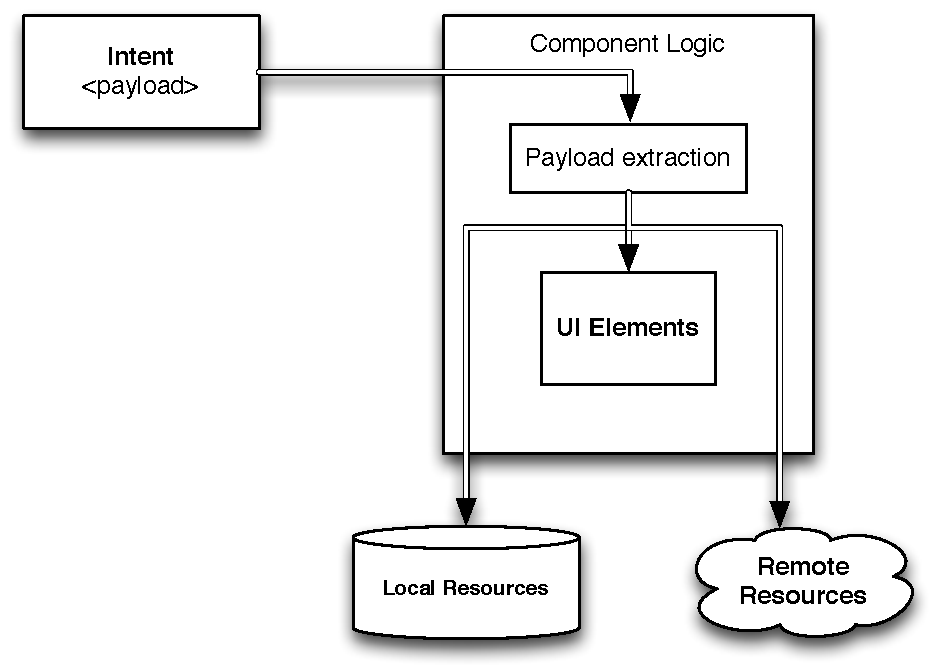
\includegraphics[width=0.5\textwidth]{images/paths.pdf}
%  \caption{Attack scenario \label{fig:paths}}
%\end{figure}
%
%Our tool discovers these sensitive paths through static analysis of an activity's code.
%To prove that the activity is exploitable along these paths, an additional step
%is needed. In fact, the existence of a path does not necessarily imply that run time
%execution of the activity will run along that path. Thus an additional problem we deal
%with this paper is that of finding such feasible paths.
%
%To this end, we design an analyzer that is able to track the path of intent data from
%sources corresponding to intent receivers to sinks corresponding
%to method calls and APIs used to send the data to the network, to databases,
%or to UI elements. Once such a path is identified, our tool automatically
%produces an intent example that can exploit that path.


% !TEX root =  ../main.tex
\section{Approach}
\label{sec:approach}


In this section, we provide an overview of our approach for automatically generating exploits as proofs of application vulnerabilities.

\subsection{Problem Formulation and Approach Overview} We formulate the problem as follows. Let the \textit{state} of an application at a particular point in the program be defined as a set of (variable, value) pairs $V = \{(v_1, a_1), (v_2, a_2), ...,$ \\
$ (v_n, a_n)\}$ visible at that point during execution. 
% Obviously, for every point in the program, there can be many possible states during execution. These states depend on the variable values at the \textit{source} statements, on the paths from those statements to the program points, and on the operations over the variable values along those paths.
To successfully launch an exploit on a specific \textit{sink}, an attacker needs to induce a state of the attacker's choosing at that sink. We denote this state by \textit{exploit state} and represent it with a set of (variable, value) pairs $V_E = \{(v_{e1}, b_1) (v_{e2}, b_2) ..., (v_{em}, b_m)\}$, where the variables $v_{ei}$ represent the parameters of the sink statement. Furthermore, to be able to induce state $V_E$ at the sink, the attacker can only use the partial control over the program input state at the \textit{source} statements defined as a set of (variable, value) pairs $V_I = \{(v_{i1}, c_1), (v_{i2}, c_2) ..., (v_{in}, c_n)\}$. Therefore, from an attacker's perspective, the problem can be stated as follows: can he determine a state $V_I$ at one or more \textit{source} statements, which induces a state $V_E$ at a targeted sink statement?

From a defensive and application vetting perspective, the following considerations complicate matters further.
\begin{enumerate}
	\item \emph{Ubiquity and number of sinks}. In general, there can be many sink statements of interest to an attacker in an application and they can be located anywhere inside that application. Thus, a robust method for identifying vulnerabilities must conservatively consider every point in the program as a possible \textit{sink} statement, even though in reality attackers are more likely prone to target only a certain type of statements.
	\item \emph{Type of exploits}. In general, there can be many possible exploit states $V_E$ for each sink statement. Consider for example a statement that creates a query to a local database. If an attacker has control over the application state at that  statement, there can be many exploit states $V_E$ at his disposal, each of which performs a different type of SQL injection. 
	Thus, a robust method for identifying vulnerabilities must not rely on assumptions about specific exploit states but must easily account for any possible exploit state $V_E$ at any point in the program.
\end{enumerate}

After these considerations, we state the problem as follows. Given any point $p$ in the program and given an arbitrary exploit state $V_E$ in that point in the program, can we automatically determine if there exists a state $V_I$ at the \textit{source} statements that induces $V_E$ in $p$ when the program executes? If the state $V_I$ exists, can we automatically determine it? Once such a state is determined, it then serves as a proof of vulnerability, since it can be easily induced in the component source statements by an attacker app, which sends a malicious intent crafted using $V_I$. 

To answer these questions, the relationship between the application state at any point in the program and the application state $V_I$ at the source statements must be made explicit. The discovery of such relationship and its modeling as a function $F$, such that we can automatically compute $V_I$ as $V_I = F(V_E)$ is at the core of our approach. We highlight at this point that depending on the operations along the execution paths there may exist several states $V_I$, which induce the same state $V_E$. For instance, if an attacker aims at inducing the state $V_E = \{ url, ``http://malicious.example.com''\}$ in line 19 of Figure \ref{lst:example}, there can be many possible states $V_I$ after the \textit{source} statement at line 5, having that value for the variable $url$ and different values for the variables $path$ and user. Our approach discovers all these possible states. 

At a high level, the steps of our approach are as follows:
\begin{enumerate}
	\item \textbf{Path computation}. Considering that every program point $p$ may be a sink statement, the paths between the \textit{source} statements and every point in the program are computed using a combination of taint propagation and static data flow analysis. 
	\item \textbf{Symbolic execution}. After the path computation step, symbolic execution over the paths is performed to derive the set of constraints imposed over the variable values along those paths. At the end of this step, for every program point $p$, a logic formula $F_p$ is created, whose variables correspond to program variables and whose terms correspond to the program statements that modify those variables. Thus, $F_p$ represents the relationship between the input state $V_I$ and the application state in $p$.
	\item \textbf{Exploit generation}. Given a point $p$ in the program with the corresponding formula $F_p$, and an arbitrary exploit state $V_E$ for that point, a new formula is created as $F$ = $F_p \wedge F_E$, where $F_E$ is a formula representing $V_E$. Next, the formula $F$ is translated into a form suitable for an off the shelf solver and solved for the variables of the state $V_I$. 
\end{enumerate}

In the exploit generation step, the formula $F_p$, which represents the relationship between the state $V_I$ and the program state in point $p$, is joined with the constraints over the variable values desired by an attacker at the point $p$. Thus, if a solution exists, it must satisfy both sets of constraints. In the rest of this section, we describe each of these steps and their challenges in more detail. 

\subsection{Path Computation}
Path computation deals with the identification of all the possible execution paths from a source statement to any program point $p$.  This task can be modeled as a data-flow problem where path information is collected inside facts associated with each point in the program. However, in the context of Android, such data-flow analysis must account for the peculiarities of the Android environment, described next.

\noindent
\textbf{Interprocedural data-flow analysis}. Android applications written in Java use method calls heavily. Therefore, any analysis framework must provide strong support for interprocedural data-flow analysis. Providing such support may be challenging, especially when identifying paths through deep sequences of method calls as well as recursive method calls. An additional challenge is posed by calls to library methods, which can largely increase the amount of code to analyze. In addition, in Android this problem is further exacerbated by the presence of native method calls over JNI with the control flow involving native code.

To deal with these challenges, we first divide the methods into two sets: user-defined and libraries. Next, a control-flow supergraph of the user-defined methods is created by the data-flow analysis framework. In this supergraph, the call sites are joined with callee definitions and callees' exit sites are joined back with the call sites. We show a portion of the supergraph built for our example in Figure~\ref{fig:supergraph}, where each node corresponds to a statement and is labeled with the line number from code listing \ref{lst:example}. 

The supergraph provides a uniform representation of the control flow across different methods and is therefore well suited for interprocedural analysis. In addition, library methods are represented as single nodes inside it, that is their body is not included in the supergraph. This choice, while potentially reducing the precision of the approach, considerably reduces the size of the supergraph and provides clear performance advantages. To limit this imprecision, we summarize the operations of the most commonly used library methods (i.e., string manipulations) with a library of constraints (described later in this section), which can be used in the formula $F_p$.

\noindent
\textbf{Path explosion}. Path explosion is a common problem when performing data-flow analysis that additionally becomes even more acute in an interprocedural context. To further limit the size of the supergraph and reduce the number of paths, we perform a preliminary \textit{taint propagation} step, which identifies the set of statements that use attacker-provided values or values derived by them and the set of statements whose execution is independent from an attacker. We include only the former set in the subsequent analysis.

In Figure \ref{fig:supergraph}, the nodes in green background represent statements that use tainted variables, while those in white background represent the rest of the statements. The source statements are represented in blue background. We note that for space reasons, not every statement is shown in Figure \ref{fig:supergraph}. 

\begin{figure*}[t]
  \centering
    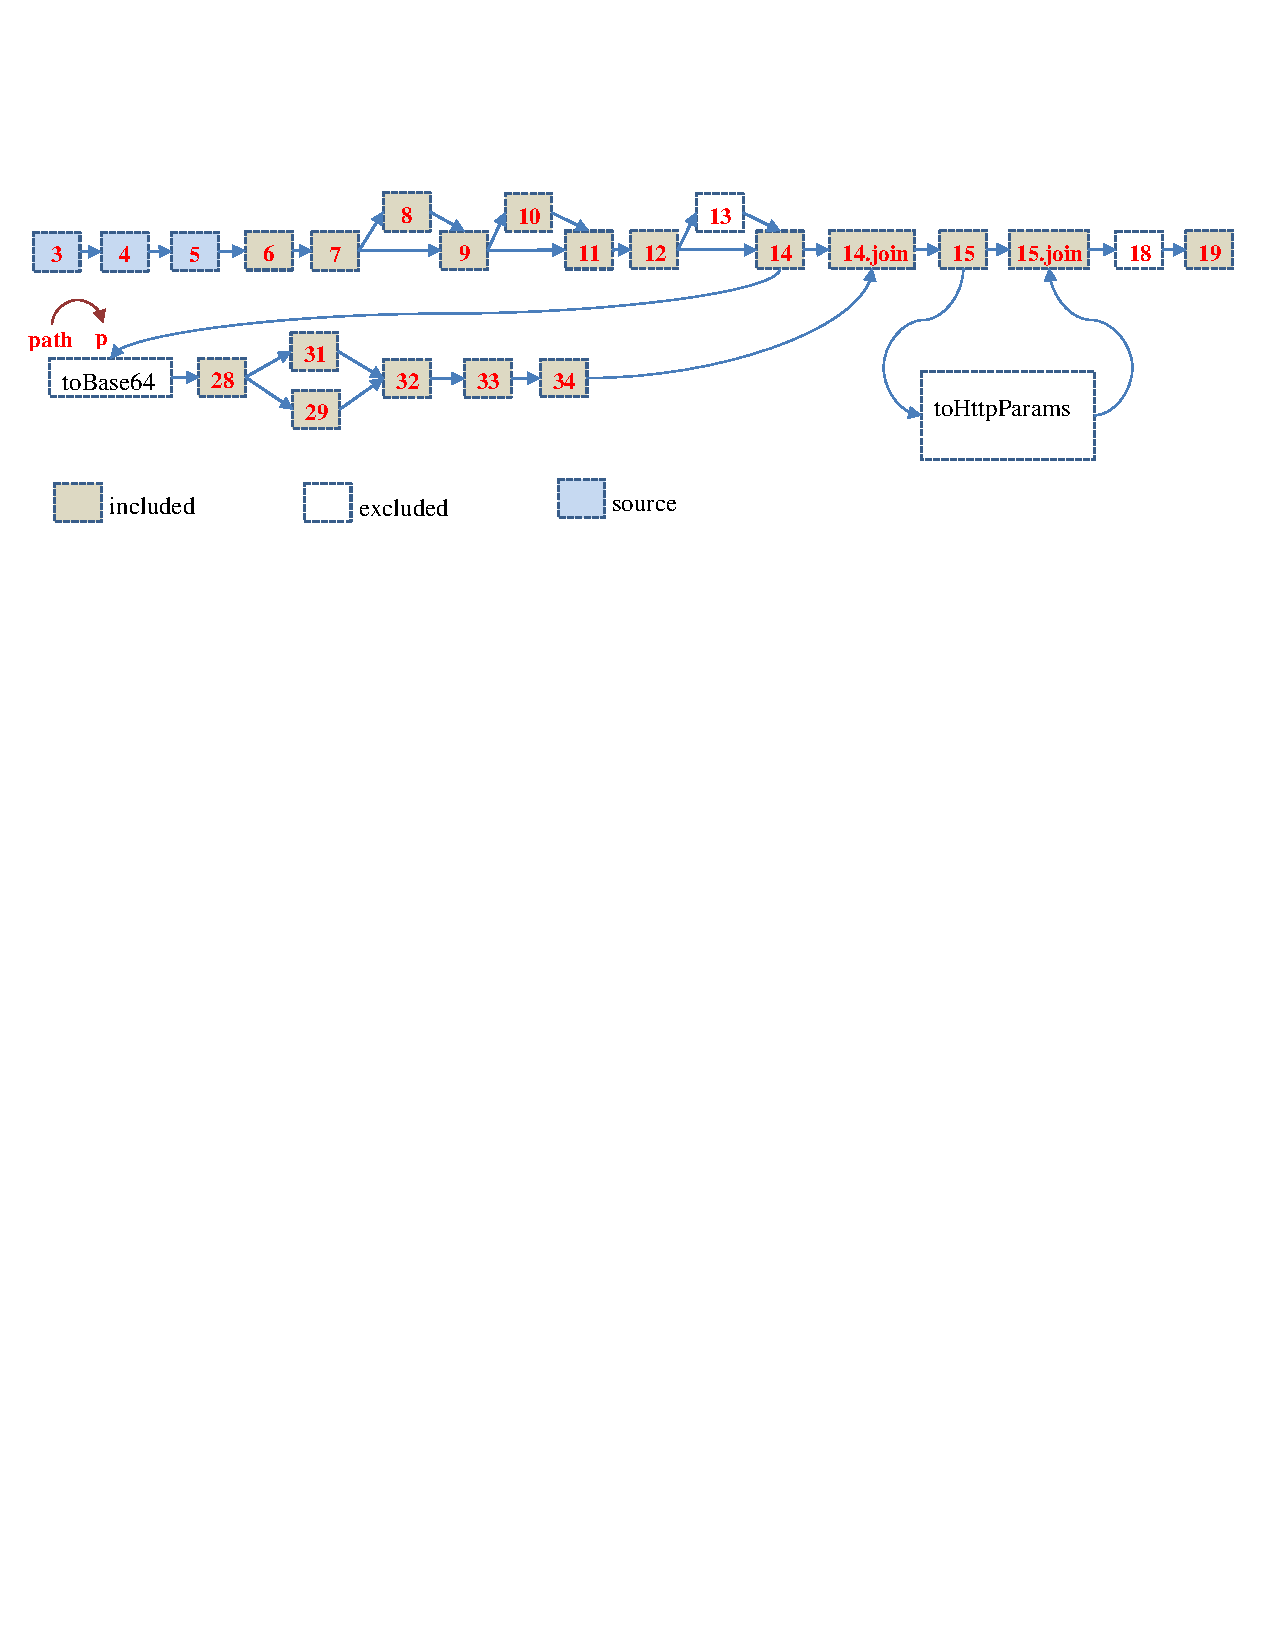
\includegraphics[width=4in]{./images/supergraph.pdf}
  \caption{Supergraph built by the analysis framework. \label{fig:supergraph}}
 \end{figure*}

\noindent
\textbf{Android application model}. An additional challenge is posed by the asynchronous nature of the Android framework and its event-guided application execution, including various callbacks. Common events are, for example, component stopping or destruction based on user-events or system-wide events, such as low memory or battery power. This execution model poses challenges in the determination of all the possible paths through which data may flow, by breaking some paths into different methods, which are not connected in the supergraph.

In our approach, we consider these methods independently: as described in detail in Section~\ref{sec:implementation} we consider each statement that extracts data from an intent as a separate \textit{source} statement and do not follow possible paths across methods that cannot be linked in the supergraph. While this choice may miss some paths, we note that a large number of these event-based method calls deals with saving the state of a component and restoring it when the component is resumed. Thus, in these cases there is no loss of information about paths and variable values.

After the preliminary step of taint propagation, the data flow analysis framework proceeds to traverse the supergraph and to collect for every point in the program the paths reaching that point from the source. The supergraph traversal starts from the source statements and adds statements to each list until a fix point is reached, and no additional statements are added to any of the lists of any program point. During this traversal, the nodes that do not use tainted variables are ignored. 


\subsection{Symbolic execution} Once the data-flow analysis framework collects all the paths for every program point, symbolic execution is used to create a formula of constraints for that point. In particular, for every program point, the list of statements is consulted and every statement different from a branching statement is added as a constraint to a symbolic formula. At the end of this step, for each program point we obtain the symbolic formula $F_p$, which models the relationship between $V_I$ and its state in that program point. 

\begin{figure}[h]
  \centering
		\begin{tabular}{lll}
			$F_p$  & $\rightarrow$ & $F_{p} \vee conj \ \vert \ conj$ \\
			$conj$ & $\rightarrow$ & $(conj \wedge term)\ \vert\ term$ \\
			$term$ & $\rightarrow$ & $stat\ \vert\ \neg stat$ \\
			$stat$ & $\rightarrow$ & $statement\ \vert\ var == statement$\\
			$statement$ & $\rightarrow$ & $statement\ +\ single\_stat\ \vert\ single\_stat$\\
			$single\_stat$ & $\rightarrow$ & $var\ \vert\ constant\ \vert\ lib\_method$ \\
			$lib\_method$ & $\rightarrow$ & $solv\_stat\ \vert\ nonsolv\_stat$ \\
		\end{tabular}
  	\caption{Grammar of Symbolic Formula}
	\label{fig:grammar}
 \end{figure}

The syntax of the symbolic formulas used in our approach is described by the grammar listed in Figure \ref{fig:grammar}. 
In particular, the symbol $solv\_stat$ represents statements and library methods whose operations semantics can be modeled by the solver used in the exploit generation step (see Section \ref{section:kaluzaTranslation}). These include string manipulation methods (e.g., \emph{host.contains(``example.com'')}).
The symbol $nonsolv\_stat$ represents statements and library methods whose semantics cannot be modeled by the solver. Finally, $var$ represents tainted variables, $constant$ represents constant strings, while the ``$+$'' symbol represents string concatenation. For instance, the formula $F_p$ related to the sink statement on line 20 of Figure \ref{lst:example} is derived as:

\scriptsize
($host.contains("example.com") \wedge url$$==$$"http$://$"+host+"/"$)$\bigvee$ \\
(! $host.contains("example.com") \wedge url$$==$$"http$://$www.example.com/"$)
\normalsize
We note that each term in the symbolic formula represents a statement along the path, while each new path created by a branching statements is represented using a disjunction. Assignment operations in the code are modeled using equality constraints, in order to capture the equality conditions between two expressions. 

% \noindent
% \textbf{Variable name preservation}. We highlight at this point the main difference of our approach with classic symbolic execution. In classic symbolic execution, symbolic expressions are used to represent program variable values. For instance, suppose the expression $x=y+z$ is present in the program and $y$ and $z$ are the symbolic input variables. Then, all the uses of the definition of $x$ are replaced by the symbolic expression $y+z$. In our approach, however, the main goal is to join the formula $F_p$ with the exploit state $V_E$ at the point $p$. Therefore, since $V_E$ is represented in terms of the variable names at point $p$, we need to preserve the names of the variables and indeed the chain of assignments and aliasing from the source statements to point $p$. 

% To capture such aliasing relations (for instance, those that occurs between concrete arguments of method calls and formal parameters of those method definitions), we use the production of the grammar that derives the string $\boldmath{var}\ ==\ \boldmath{var}$. For instance, in our example, an aliasing relation occurs between the variables $path$ and $p$. This aliasing relation is shown in the graph in Figure \ref{fig:supergraph} by the arrow $path \rightarrow p$, and it is represented in the symbolic formula by the term $path == p$. 

% \noindent
% \textbf{Library Methods}. As previously mentioned, we consider library methods as unit statements during path computation. However, as shown by the last rule of the grammar, during symbolic execution we divide the library methods in two sets, namely \emph{solvable statements} ($solv\_stat$) and \emph{non solvable statements} ($nonsolv\_stat$). The former includes statements that manipulate strings, which the solver can deal with (e.g., \emph{host.contains(``example.com'')}), while the latter includes statements that cannot be processed by the solver (e.g., \emph{InputStream.read(p)}). This type of statements are included in the formula and the result given by the solver for the variables in the latter set will be the whole domain (*). For instance, the solver reports that the variable $bytes$ in line 32 can be anything. 

\noindent
\textbf{Loops}. One of the main issues in symbolic execution is dealing with loops. In fact, even a single loop can generate a large number of execution paths depending on different number of iterations and paths inside the loop. Since the number of loop iterations is unknown during static analysis, a common strategy is to place an upper bound over the number of times a loop is executed symbolically. In our approach, we execute each loop symbolically one time. This choice allows us to cover the loop body statements while still having an acceptable performance.




% 3) Untainted variables. These can appear only inside statements that use tainted variables as well (because we filter out all the other statements. In the end, the solution given by the solver for the untainted variables is the whole domain (*). So how do they appear in the formula?\\




%Since the second clause does not lead to a propagation of $hostname$ to the sink, the solver is
%able to generate an exploit satisfying the first constraint. The solution will be $example.com@$ where the ``$@$'' symbol stays for any %string.

%\lstset{numbers=left, basicstyle=\ttfamily\scriptsize, breaklines=true}
%\begin{lstlisting}
%$filename.contains("..") ->
%   $filename.replace("..", ".")
%$filename.length > 0
%$filename := "/data/data/com.example/public/" + $filename;
%\end{lstlisting}




\subsection{Exploit Generation}
The input the exploit generation step, is a program point $p$, the corresponding formula $F_p$ and a set of assignments representing the exploit state $V_E$. The first operation of this step is the translation of the symbolic formula $F_p$ into the solver's language. In particular, for each member of the $solv\_stat$ statements, we create a set of constraints in the language of the solver, which model the behavior of that statement (for more details about this task, see Section \ref{sec:implementation}). The members of the $unsolv\_stat$ statements are modeled with a particular operator in the solver's language that returns the whole domain of values for the variable.



%In our threat model we focus our attention on intent payloads, not on their nature or kind: we consider payload
%contents to be the unique input that a possible attacker can exploit in order to gain control of the application environment. By doing this, differently from Chex, we do not consider attack concerning sequences of Intent messages and their interaction, but we focus our efforts on a deeper analysis about the consequences of a single intent reaction of the vulnerable application.


%The input received by an application component via an intent is a set of variables, each having a range of possible values in the domain determined by the variable type. We denote a set of such variables as $I_a=\{i_{a1}, i_{a2}, ..., i_{an}\}$. Further, we call the statements of the application component where such variables are first received \textit{source} statements. In our running example in Section~\ref{sec:running-example}, lines 4 and 6 in Figure~\ref{fig:example-code} are \textit{source} statements. In addition to the set $I_a$, the application component may also use other variables, which are not input via an intent and may or may not be under the control of an attacker. For instance, variables such as device identifiers and application database data belong to this category. We denote this set of variables with $I_b=\{i_{b1}, i_{b2}, ..., i_{bn}\}$. In the following, we assume that the attacker does not control variables in the set $I_b$, even though in practice there may exist cases where the attacker may have partial control over the set $I_b$ or obtain the values those variables from the environment.
%
%Conceptually, the application component processes the input variables according to its own logic, and produces in output a new set of variables, which we denote as $O=\{o_1, o_2, ..., o_m\}$. Correspondingly, any statements in the program where data may trigger a malicious abuse will be called a \textit{sink} statements (e.g. line 14 in Figure~\ref{fig:example}.b). Using this notation, an application component can be described formally as a function $F: I_a \cup I_b \rightarrow O$.
%
%%Conceptually, the function $F$ represents both the application logic proper and eventual data validation and sanitization operations.
%%We have not started talking about paths yet. But depending on the application, several such functions may exist for the same input, because there may be different reachable sinks.
%
%In an intent-spoofing attack, the goal of an attacker is to induce an application component to produce a desired output $O_m=F(I_a \cup I_b)$ by appropriately crafting $I_a$, such that the variables in the output $O_m$ are parameters to sensitive operations (e.g. they are values of UI elements, data being sent over the network to a server, etc.).
%
%Ideally, we want to verify that, for every possible $O_m$ desired by an attacker, there is no input $I_a$ such that $F(I_a \cup I_b)=O_m$. In practice, given that there are usually multiple sinks, and multiple potential malicious output sets $O_m$ desired by an attacker, determining every possible malicious set $O_m$ for every sink is hard. However, $O_m$ is a subset of the set of all possible outputs. So we can first determine all source-to-sink paths in the application, and then compute the set of all possible outputs via symbolic evaluation (with some approximation). At this point, we can provide a ``proof of concept'' exploit, by automatically computing a malicious input string, given the desired output.

%\begin{table*}[t]
%\begin{tabular}{|l|l|l|l|}
%\hline
%\textbf{Category} & \textbf{Pattern} & \textbf{Description} & \textbf{Taint Action} \\
%\hline
%Simple  &  $var=var_t\ op ...\ op \ var_t$ & Assignment with no function calls on & $taint(var)$ \\
%   Statement      &                                & RHS and at least one tainted & \\
%                  &                                & variable on the RHS & \\
%\hline
%User-defined     &  $var=foo(var_t,...)$  & User-defined procedure on the & $ taint(formal)$,\\
%function call    &                        & RHS of an assignment.      & $(taint(var)\ if\ isTainted(return))$ \\
%\hline
%User-defined    &  $foo(var, var_t,...)$  & User-defined procedure call & taint(stmt) \&\& taint(formal)\\
%function call    &       &    & $taint(var)$\\
%\hline
%API function  & $a=api(var_t,...)$ & API procedure on the RHS of an assignment & taint(var) \\
%   call               & $api(var, var_t,...)$ & API procedure call & $taint(var)$\\
%\hline
%\end{tabular}
%\caption{Taint Policy}
%\label{tab:Taint}
%\end{table*}

%\subsection{Path Identification}
%The first task of our approach is identification of all the different paths among sources and sinks. To do so, we build a static taint analysis framework to keep track of the variables in set $I_a$ and statements affected by those variables (as they are the only ones that the attacker can affect in our threat model).
%
%We proceed as follows. A taint is introduced for each variable whose value is derived from the set of variables $I_a$, i.e. for each variable whose value is set by the get methods of the Intent class. For instance, with respect to Fig. \ref{fig:example-code}, a taint is introduced initially for each of the variables \textit{url} and \textit{path}.
%
%At this point, the taint is propagated according to the policy summarized in Table \ref{tab:Taint}, where we denote with $var$ an untainted variable, with $var_t$ a tainted variable, $taint(var)$ the taint action on a variable $var$,and with ($taint(formal)$), the tainting action on a formal parameter of a function definition. For brevity, we report only the cases in which the taints are propagated.
%
%%TODO how do we support the assertion that the APIs are safe?
%As shown in Table \ref{tab:Taint}, the variables appearing on the LHS of an assignment containing no function calls are tainted if there exists at least a tainted variable on the RHS of that assignment. For user-defined functions having tainted variables as arguments, we propagate the taint to the corresponding formal parameter ($taint(formal)$) and taint the variable on the LHS of the assignment if the return value of the function is tainted.
%If, however, an untainted variable is passed as input to the function and tainted inside that function, that taint is preserved after exiting the function. Finally, for API function calls, we do not propagate the taints inside the functions' body, based on an assumption that they are generally safe, and also for performance reasons, which will be discussed in Section \ref{sec:implementation}. However, we make the conservative assumption that eventual untainted variables will be affected by the function call, and taint them.
%
%Taint propagation proceeds along the interprocedural control flow graph of a component and stops when a \textit{sink} statement is reached. Currently, sink statements are defined manually, and include calls to API procedures that deal with setting the values of UI elements and sending data over the network.
%
%At the end of taint analysis, the variables of an application component are partitioned into two sets: those whose values and execution may be potentially affected by the attacker's input, and those whose values and execution are not affected by an attacker's input. In addition, the statements are also partitioned into two similar sets: those statements that contain tainted variables and those statements that do not contain tainted variables. Intuitively, the execution of the former can be potentially affected by an attacker's malicious input, while execution of the latter cannot be affected by an attacker's input.
%
%\subsection{Path Computations}
%
%The described taint propagation is only the first step towards characterizing a component as a function $F$. To derive a model about the possible outputs at the sinks, we use symbolic execution over the paths discovered by the taint analysis step and employing the variables in $I_a$ as symbolic values.
%
%
%One of the main challenges of symbolic execution is \textit{path explosion}, where the paths to be considered may increase exponentially. An additional  challenge is represented by the presence of procedures, each of which defines a new execution context with its own control flow graph. Similarly to the taint analysis, in the presence of procedures, a symbolic execution framework must solve additional problems, such as variables with the same name defined in different contexts, correspondence between actual arguments of a procedure call and formal parameters of a procedure definition, and the relationship between values returned by the callee and variables of the caller.
%
%All the above challenges are exacerbated by the presence of calls to the framework APIs. In fact, due to their size and interconnectedness, the number of paths can rise very rapidly, and the complex patterns between arguments, formal parameters, and return values contribute to render symbolic execution intractable.
%
%To be able to symbolically execute the program across procedures, we construct a control flow super-graph that combines the control flow graphs of the those procedures and establishes relations between call arguments and formal parameters and between callee return values and variables at the caller site.
%In addition, to address the path explosion, in constructing this super-graph we make the following choices: 1) we prune the graph from the untainted statements and 2) similarly to taint analysis, we treat API calls as atomic instructions and do not expand them further. The former choice allows us to reduce the size of the graph, while preserving the precision of the symbolic execution as much as possible. For instance, the statement at line 6 in Fig. \ref{fig:example-code}, which is not tainted, is removed from the super-graph.
%The latter choice forces us to obtain only approximate results.
%
%After the reduced super-graph is obtained, we traverse it starting from the \textit{source statements} and, for every statement, add a term to a symbolic formula, which represents the computations on the variables of $I_a$ (See Section \ref{sec:implementation}).
%
%In general, tainted statements contain also untainted variables whose values cannot be affected by the variables in the input set $I_a$. For instance, the line 7 of the code in Fig. \ref{fig:example-code} contains a call to a user-defined procedure that has the untainted variable $user\_id$ as argument. In our approach, we include these variables in the formula. In fact, when the formula is solved, the values of these variables will be the entire domain.
%
%The symbolic execution stops when a \textit{sink} statement is encountered. For each sink, we therefore produce several conjunctive formulas, each corresponding to a computation path from a \textit{source} statement to a \textit{sink statement}. These formulas represent effectively the function $F$, which models the values computed at the sink statements starting from the variables in the input set $I_a$.
%
%\subsection{Exploit Generation}
%
%Once a symbolic formula $F$ representing the constraints and computations along a path is obtained, the next step in our approach is to attempt to generate an exploit using $F$. In fact, the existence of a path does not imply a vulnerability, since the path may contain validation and sanitization checks. Therefore, we attempt to generate an exploit in order to test for, and provide the proof of, the existence of an actual vulnerability.
%
%To generate an exploit, we use a two-step strategy. First, we use a constraint solver to solve the formula $F$ for a path without any constraints over the output variables at the sinks. In other words, we ask the solver to provide all of the input values that produce any output at all. Guided by these first results, we augment the symbolic formula with constraints that restrict the output values to a malicious set $O_m$. The solution to this augmented formula contains the set $I_a$ of malicious input values.
%
%% \subsection{Assumptions and limitations}
%
%% % TODO maybe this should be merged back somewhere else
%% In our approach has a few limitations and simplifying assumptions. First, our current implementation deals only with string variables and string operations. However, from our experience, most of the intent data carry string variables. Also, this is an implementation issue, our approach can be extended to handle other types of data.


%% !TEX root =  ../main.tex
\section{Elements of the analysis}
\label{sec:analysis}


% !TEX root =  ../main.tex
\section{Implementation}
\label{sec:implementation}


In this section, we discuss the implementation of the different steps of our approach.

{\color{orange}
\subsection{Implementation Background}
In this subsection, we provide a short background on two techniques and tools that we used in our implementation, namely the IFDS framework and Kaluza. 

\noindent
\textbf{IFDS framework}.
IFDS is a framework for interprocedural data flow analysis that transforms dataflow problems into graph reachability problems \cite{ifds,Bodden:2012:IDA:2259051.2259052}. This framework  is particularly efficient in dealing with interprocedural data flow analysis, and highly customizable to represent different data flow problems. The framework takes care automatically of several general analysis tasks, such as
determination of valid paths on the control flow supergraph (i.e., paths that can potentially be executed at runtime) and of fact propagation. However, to solve a specific analysis problem, it is necessary to formulate it appropriately as an instance of an IFDS problem. In practice, this means defining the analysis information contained in the data-flow \emph{facts} as well as the \emph{rules} that update that information for every node in the control flow supergraph. 

\noindent
\textbf{Kaluza}.
Kaluza is an efficient solver for formulas containing string variables and constraints in the form of string equalities, substring operations, numeric constraints over string lengths, and so on  \cite{kaluza,kaluzaKudzu}. Kaluza natively supports a set of string operations, such as string concatenation, equality, and length equality. \todo{W2.5 Added reference to the Kudzu (Kaluza) paper.} 

} \todo{W1.5. Added implementation background section for IFDS and Kaluza.}

\subsection{Path Computation}
As mentioned previously, the problem of path computation is a typical interprocedural data-flow problem. In our approach, we model this problem as an instance of an interprocedural, finite, distributive, subsets problem (IFDS). This framework is build on top of Soot, a Java optimization framework, due to the many analysis facilities it provides \cite{heros,Bodden:2012:IDA:2259051.2259052,Vallee-Rai:1999:SJB:781995.782008}. In addition, we use the Heros Soot plugin, which provides a fully context-sensitive implementation of the IFDS framework \cite{heros}.
\todo{W2.6}

To prepare the application for use with Soot and HEROS, the Dalvik bytecode is first transformed into Soot's intermediate representation language Jimple. While in theory this transformation may be lossy and not retrieve the original code, these losses are negligible. Jimple is particularly suited to our task, since it provides a three-address and single assignment representation of the code, making it easier to derive the information about paths and perform symbolic execution. In addition, the Soot framework provides many ready-to-use capabilities for code analysis.

In our implementation, we model the preliminary taint propagation step as a data-flow problem as well, and incorporate it into the IFDS instance problem of path computation. This removes the need for running this step separately and improves the efficiency of our implementation. Before proceeding further, we provide a short review of the IFDS framework.

% IFDS relies on a control flow supergraph similar described in Section \ref{sec:approach}. 
% After a user defines the analysis information contained inside a fact and the update rules for different types of nodes, the IFDS framework then proceeds to traverse the supergraph and use those rules to update facts with new information. The graph traversal stops when a fixpoint is reached and no new information can be added to any facts.


\noindent
\textbf{Source statements detection}.
The first step in defining the problem as an IFDS instance is the specification of the \textit{source statements}, which constitute the IFDS analysis entry points. To detect these entry points, a full scan of the Jimple representation of the program is performed and the instructions that perform Intents and Bundle payload extraction (e.g. $getStringExtra$) are identified. Since the set of API calls that Android provides to extract Intent payloads is limited, we use an exhaustive list of method signatures for this task.
%What does the sentence: "A step further...." mean?
A step further is made in order to reconcile extractions of different payload pieces conceptually belonging
 to the same Intent message. 
 After this detection, the program variables whose value is defined in the entry points serve as the initial taint variables. These are indeed the variables appearing in the state $V_I$, whose value can be set by an attacker.
%In most of the cases, this extraction is performed in the $onCreate$ or in the $onBind$ methods, which are the set-up methods for both Android Activities and Services.
% Practically, this means that we will have a direct connection between an attack stimulation (sending an intent message) and the vulnerable code fragments that use them.


%We are not using these entry points later. REMOVE
% To represent an entry point, we use a data structure populated with information about the Android component in which the extractions
% were encountered, the method in which the single piece was first assigned complete with the exact location
% in the method body. An entry point for the payload piece $host$ in the example proposed in Figure~\ref{lst:example} is shown below:
% \begin{verbatim}
%   EntryPoint =
%    {
%      name: "host",
%      component: SendActivity,
%      method: SendActivity$onCreate(),
%      location: line 3,
%      statement:
%       String host = intent.getStringExtra("host");
%    }
% \end{verbatim}
% In this case, the following steps of the analysis, consider the variable $host$ as the tainted variable
% from the \textit{source} statement. %The path identification and computation steps are aimed to find a path between
%variable $url$ and a vulnerable sink, in addition to a value to this variable that makes
%such path traversable.

\noindent
\textbf{Path Computation and Taint Propagation}.
The next step in modeling our problem as an IFDS instance, is to define the information contained inside the dataflow facts and how this information is updated for the different nodes of the supergraph. In our implementation, we use a special definition of a \emph{fact}, which contains both taint propagation and path information. Thus, a \emph{fact} is defined as tuple $F = (input\_vars, tainted\_vars, statements, cond\_statments)$, where $input\_vars$ represents variables from the state $V_I$ whose values is defined in the source statements (namely predefined Android API statements that extract values from intents), $tainted\_vars$ is a set of variables representing the tainted variables, $statements$, is the list of statements from the source statement to the current point in the program, and $cond\_statements$, is the list of all the conditional statements from the source statement to the current point in the program. 

{\color{orange}
Thus, for every program point, the fact associated with that point contains the list of input variables, the list of tainted variables visible in that point, as well as a list of statements contained in the paths from the source statements to that program point. The taint is therefore propagated to a variable by adding that variable to the list.
} \todo{W2.3a}
%Do we need this? We do not use it later in the discussion
  %In addition, each fact stores the name of the component containing the source statement as well as the name, the type and the method signature containing the source statement. 
% For instance, when the analysis reaches line 3 in Figure \ref{lst:example} where the $host$ variable is extracted from the intent, a new fact $Fact$ is created:

% \begin{verbatim}
% Fact = { input-variable: "host",
%   tainted-variables: "host"
%   statements: host=
%         intent.getStringExtra("hostname")
%   conditional-statements: <empty>
%   context: line 3 }
% \end{verbatim}

During analysis, the IFDS framework takes care of traversing the supergraph and update the facts associated with each node using user-defined \emph{rules}. These rules are different for every node and described below.
\begin{itemize}
 \item \textit{Normal Rules:} These functions define how fact information is updated for nodes different from method calls. In this case, we add a statement to the $statements$ list if: either the $input\_vars$ or one of the $tainted$ variables is used by the statement. A new variable is added to the $tainted$ set if its value is obtained by using one of the $input\_vars$ or a tainted variable. \todo{W2.3b.}
 \item \textit{Call Rules:} These rules define how fact information is updated for procedure calls. In this case, the call statement is added to the $statements$ list, if the $input\_var$ or one of the tainted variables are contained in the list of arguments. In addition, this rule is used to add to the set of tainted variables the formal parameters of the callee that correspond to tainted variables in the call.
 \item \textit{Return Rules:} The purpose of a return rule is to propagate the information discovered inside the body of a called method to the caller. Using this rule, the taint information is therefore propagated to the variables at the caller site. For instance, since the return value of the method $toBase64$ is tainted, the variable $b64File$ is added to the list of tainted variables.
\end{itemize}
% Both normal and call rules serve also to create a new fact, when a method that extracts data from an intent is encountered.

% % \todo{Added}
% % For instance, the fact $F$ is created when the analysis reaches line 4. The statement at line 5 where the $filename$ variable is used, is also added to the $tainted-statements$ set. In addition, the $b64File$ name is added to the set of $tainted$ in $F$, since the statement contains the $filename$ on the right hand of the assignment.
% % The statement at line 7 is added as well to the $tainted-statements$, since the alias $b64File$ is matched. The variable $httpPar$ is also added to the $tainted$ set, since $b64File$ now appears on the right hand side of the statement.

% After the definition of these rules is provided, the IFDS framework traverses the super-graph and executed them depending on the type of statements encountered. For instance, if the statements contains a procedure call, call rules are executed. We added an exception to this behavior in our implementation: When the statement contains a library method call, we execute normal rules rather than call rules to prevent the IFDS framework from traversing the body of those calls.

\subsection{Symbolic Execution Implementation}
Given the paths identified inside the facts by the previous step, we match each statement to one of the productions of the symbolic formula grammar described in Section \ref{sec:approach} and add it as a term to the rest of the formula. In particular, the rules for each of the productions are described below. {\color{orange} In this step, we also perform variable name rewriting, to $flatten$ the objects and to extract constraints among $String$ variables. This renaming is performed by prepending to the name of a variable, the name of the method it is declared in and the name of the corresponding object (if available). For instance, the variable $p$ inside the function $toBase64$ is renamed to $toBase64\_p$.} \todo{W2.2b}
\begin{itemize}
\item \textit{Assignment statements:} Every assignment statement in the path is transformed into an equality constraint.
\item \textit{Branching statements:} For every branching statement, symbolic execution is split into two paths and the condition of the branching statement is added to the true branch, while its negation is added to the false branch.
For instance, when the $if$ statement in line 28 of Fig. \ref{lst:example} is encountered, the condition $toBase64\_p==null \| toBase64\_p==``''$ is added to the formula representing the path that contains the $then$ part of the statement, while the condition $!(toBase64\_p==null \| toBase64\_p==``'')$ is added to the path that contains the $else$ part of the statement.
\item \textit{User-defined procedure calls:} When a call to a user defined method is encountered, we first rename the local variables of the method by prepending the name of the function to avoid duplicates, then add equality constraints between arguments and formal parameters. Next, we proceed to symbolically execute the function. For instance, since the variable $file$ is passed as an argument to $toBase64$, we add the constraint $``file == toBase64\_p''$ to the formula. If the function returns a value that is assigned to a variable, we add an equality condition between them as well. For instance, the condition added after the return statement of $toBase64$ is $b64File==toBase64_b$.
\item \textit{Library method calls:} Unsolvable library method calls are replaced by a special term whose purpose is to not introduce any constraints to its arguments. 
\end{itemize}

% !TEX root =  ../main.tex

\subsection{Exploit Proof Generation}
 \label{section:kaluzaTranslation}

As mentioned previously, to generate an exploit as a malicious state input state $V_I$, we chose to use the Kaluza constraint solver. Kaluza natively supports several string operations. For other operations, not natively supported by Kaluza, a translation system for a set of Java (Jimple) standard library methods was built, which focuses on string and integer constrains. This set together with the set of operations natively supported implements the \emph{solvable} library methods previously discussed. Some examples of these custom translations are listed in Table~\ref{table:tabkaluza}, using regular definitions. 

% \begin{table}[t]
% \small
%    \centering
%     \begin{tabular}{|l|l|}
%       \hline
%       \textbf{Java} & \textbf{Kaluza formulation}\\
%       \hline
%       $a.contains("test")$ & $a == /.*test.*/$ \\
%       % \hline
%       % $a.indexOf("test")$ & $a \rightarrow T1 T2 T3$ \\
%       %             & $T1 \nrightarrow test$ \\
%       %             & $T2 \rightarrow test$ \\
%       %             & $T3 \rightarrow *$ \\
%       %             & $a\_indexOf \rightarrow Len(T1)$ \\
%       \hline
%       $new\_a = a.replace("test",$ & $a == T1 T2 T3$ \\
%        $"newTest")$ & $T2 \rightarrow test$ \\
%                       & $T4 \rightarrow newTest$ \\
%                       & $new\_a \rightarrow T1 T4 T3 $ \\
%                       & $T1 \rightarrow *$ \\
%                       & $T3 \rightarrow *$ \\
%       \hline
%     \end{tabular}
%     \caption{Kaluza constraints formulation example}
%     \label{table:tabkaluza}
%   \end{table}



\begin{table}[t]
   \centering
    \begin{tabular}{|l|l|}
      \hline
      \textbf{Java} & \textbf{Kaluza formulation}\\
      \hline
      $a.contains("test")$ & $a \in CB(/.*test.*/, 0);$ \\
      \hline
      $a.indexOf("test")$ & $a := T1 . T2;$ \\
                  & $0x0 == Len(T1);$ \\
                  & $T2 := T3 . T4;$ \\
                  & $T3 := T5 . T6;$ \\
                  & $T6 == "test";$ \\
                  & $T5 \notin CB(/test/, 0);$ \\
              & $a\_indexOf == Len(T5);$ \\
      \hline
      $new\_a = a.replace("test",$ & $a := T1 . T2;$ \\
       $"newTest")$ &  \\
                      & $T2 := T3 . T4;$ \\
                      & $T3 := T5 . T6;$ \\
                      & $T5 \in CB(/test/, 0);$ \\
                      & $T7 \in CB(/newTest/, 0);$ \\
                      & $T8 :=  T9 . T4;$ \\
                      & $T9 :=  T7 . T6;$ \\
                      & $new\_a := T1 . T8;$ \\
      \hline
    \end{tabular}
    \caption{Kaluza constraints formulation example (CB = CapturedBrack)}
    \label{table:tabkaluza}
  \end{table}

\todo{W2.4a. Reinstated Daniele's original table.}.
  %These translations rely on Kaluza regular expressions and constraints. For instance, the $String.replace$  method is translated by producing a conjunction of constraints:
  %the string ($var_a$) is divided into parts ($T1$ and $T2$ in the example) in order to identify the correct
  %string part to substitute ($T5$). The new string is then defined to contain the replaced part
  % ($T7$) in addition to the other non-matching string parts that do not need replacement.
  % A similar approach is adopted for the $indexOf$ method: instead of replacing the string, the formulation identifies the correct position of the first occurrence of the lookup string in the original string by identifying the matching string part.
  % For sake of clarity we present a line-by-line discussion of the $String.replace$ formulation.
  % Line $1$ defines the variable $\$var\_a$ as the concatenation of two substrings ($T1$ and $T2$).
  % Since the string to replace be found in the middle of the string, this first
  % splitting is not exhaustive. At Line $2$ and $3$ we proceed further splitting the substring $T2$ in three
  % pieces: $T5$, $T6$ and $T4$. Thanks to this string representation and not bounding the lengths of the pieces
  % we can handle any positioning of the replacement string.
  % At line $4$ we use $CapturedBrack$ (a regular expression helper) to explicitly declare which one is the part
  % containing the string to be replaced. Similarly at line $5$ we ensure to have a new string piece ($T7$)
  % including the replacement string.
  % The remaining constraints (Lines $6-8$) compose the new string by concatenating the string pieces,
  % including $T7$.


  % Since Java and Kaluza are both statically typed, we did not had to care about type casting
  % explicitly. For this reason the lookup of the method intended to be translated is straight forward
  % and can be done by exactly matching the method signature. The Kaluza transformation is consistent
  % in different invocation of the same  method signature.

  % It is important to note that, in general, not all of the methods included in symbolic formulas produced by the paths computation step can be translated into Kaluza. Examples include API calls with types that cannot be cast to a Kaluza type. For instance, in our example code in Figure~\ref{lst:example}, this happens with the instruction Base64Encoder.toString(bytes). Another typical example are API calls that we consider as atomic instructions.


  For library methods that can not be translated directly in Kaluza (e.g., Base64Encoder.toString(bytes)), a report is created in output, and either a Kaluza approximation of their functionality is manually built or they are represented by a special term that places no constraints on the values of their variables. An example of such approximation is the $split$ method, which is a utility function to divide a string into pieces separated by a substring given in input to the function. $Split$ returns an array, and arrays are hard to represent in Kaluza because they are defined as an unknown number of variables, while Kaluza accepts only defined numbers of variables. Our approximation consists in producing the entire string instead of an array of parts as returned value of the method.

% \begin{itemize}
%   \item \textbf{Alias binding}: by binding parameters to arguments we obtained a
% linear and simple representation of the intra-procedural flow. As we can see at Line~$1$ in the wxample, we adopted the
% method signature as namespace to local variables so to have a unique value name
% for each variable in the code flow. In order to produce this bindings we use the $<tainted>$ data structure contained in the fact.
%   \item \textbf{Constraints translation}: we implemented a class of utility
% functions to translate string comparisons methods to a formal Kaluza representation. We directly extract the comparison information from the fact's $<conditional-statemets>$ data structure. In order to correctly detect the control flow edge leading to the vulnerable statement (vulnerable sink), we locally explore the CFG (Control Flow Graph) and we possibly flip the constraint condition (Line~$2$ of the example).
% \end{itemize}

% \begin{itemize}
%   \item \textbf{Graph building}: as first step of the process, we are interested in producing an
%   unified Graph of the original control flow graph by removing all the statements that does not
%   involve any of the statements that operates or include either the \emph{base variable} or one
%   of its aliases. The resulting sub-graph is then obtained by recursively merging all the methods' graphs
%   starting from the sink to the \emph{base variable}.

%   Here below is presented a sketch of the algorithm used to obtain the desired graph.
%   Where:
%   \begin{itemize}
%   \item $graph$ is the resulting graph variable
%   \item $sink$ is the vulnerable statement
%   \item $statementsSet$ is the list of tracked statements from the IFDS analysis
%   \end{itemize}
%   The algorithms works as follows: starting from the vulnerable statement point in the code
%   the control flow graph is traversed backward (w.r.t. normal code execution order) jumping
%   from callee to callers until the \emph{entry point} variable is reached.

%   $extractMethod$ is the algorithm wrapper function taking care of managing inter-procedural calls.
%   After adding the vulnerable statement the algorithms iterates over the callees until the newly generated
%   graph has not been changed (convergence point).

%   \lstset{numbers=left, basicstyle=\ttfamily\footnotesize, caption=Subraph building., label=codelisting}
%   \begin{lstlisting}
% graph;
% sink;
% statementsSet; // list of captured statements
% extractGraph() {
%  context; // sink's method
%  contextGraph;

%  graph.addNode(sink);

%  addPredecessors(contextGraph, sink, sink);

%  repeat {
%   headMethod= methodOf(lastUpdatedHead);
%   caller= callerOf(headMethod);
%   context= methodOf(callerStmt);
%   contextGraph= extractGraph(context);

%   if (caller in statementsSet) {
%    addPredecessors(contextGraph, callerStmt, prevHead);
%   }

%  } until (graph.getHead() != lastUpdatedHead);
% }

% addPredecessors(contextGraph, currentStatement, graphHead) {
%  for (predecessor, i :
%     currentStatement.getPredecessors()) {
%    if (!currentStatement in statementsSet) {
%     addPredecessors(contextGraph, predecessor, graphHead);
%     return;
%    }
%    if (current statemet branches) {
%     if (i == 1) {
%      addNodesAndEdge(graphHead,
%         <Empty>);
%     }

%     addNodesAndEdge(predecessor, graphHead);

%     if (i == 0) {
%       addNodesAndEdge(graphHead,
%         <Empty>);
%     }
%    } else {
%      addNodesAndEdge(predecessor, graphHead);
%    }

%    addPredecessors(contextGraph, predecessor, newGraphHead);
%  }
% }

%   \end{lstlisting}
%    $addPredecessors$ iterates over statements inside a specific method body and it is in charge
%   of reconstructing intra-procedural code points from the original method's body to newly constructed graph.
%   This method is invocated from the precise program point from which the previous method was invocated
%   until the first statement in the method body.

%   The function first checks whether the current statement was tracked in the previous analysis step or not,
%   i.e. such statement affects somehow the \emph{base variable} (or one of its aliases) or not.
%   If a match is encountered and the statements is not a merging point (the graph branches),
%   the current statements is simply added to the graph and the next statement is taken in consideration.
%   If the statement is a merging point, since the then-else branches are positional in the graph semantic,
%   the right position for the next statement has to be preserved. This is obtained by checking
%   the index of the current statement in the predecessors list (0 or 1).

%   It has to be noticed that:
%   \begin{itemize}
%   \item the first statement in a method body has no predecessors
%   \item points in the code in which if-then-else blocks merges have two predecessors
%   \item all other statements have only one predecessor
%   \end{itemize}

%   $addNodesAndEdges$ method (not presented here) is a simple utility method to add the edge
%   between the two nodes in the right position.


  % In order to avoid clashes, local variable names are transformed by prefixing to them their method name.
  % For example variable $v$ of method $doSomethingElse$ presented in the example \ref{sec:graph_buinding} is transformed to
  % the variable name $doSomethingElse_v$.

After the constraint solver processes the translated formula, it provides a set of solutions for the ranges of variables in $V_I$ for which the formula $F_p \wedge V_E$ is satisfiable, {\color{blue} where $V_E$ is also expressed using the Kaluza language, which provides the opportunity to define several patterns for the values of the parameters at the sinks.} Conversely, an unsatisfiable result produced by the solver means that the vulnerable sink cannot be reached, in practice, at run-time. For instance, the following example shows a Kaluza formula derived from one of the studied applications. In this example, after ensuring that the input value $source$ length is greater than 0, the prefix is stripped out (if any) in $tmp$. This $tmp$ variable is then matched against a regular expression for validation purposes. Our tool was able to traverse the control flow graph with the Jimple representation of this code fragment, and in the end obtain the solution $444494 4944$.
\lstset{numbers=left,xleftmargin=1cm, basicstyle=\ttfamily\scriptsize, breaklines=true}
\begin{lstlisting}
$source.length > 0
$IF(source.startsWith("+1")) { $tmp := $source.substring(2, $source.length - 1) }
IF((not $source.startsWith("+1"))) { $tmp := $source }
$tmp.match("/([2-9][0-8][0-9])\ *([2-9][0-9][0-9])\ *([0-9][0-9][0-9][0-9])/")
\end{lstlisting}

\todo{W2.4b}


\subsection{Approximations and limitations}

For simplicity, we used several approximations in our approach. We discuss their impact in the following paragraphs.

\emph{Untainted input variables}. Motivated by efficiency considerations, we chose to ignore variables whose values cannot be affected by the variables input via intents. While allowing us to prune a portion of the control flow super-graph by removing statements that do not use tainted variables, this choice may also reduce the precision of our approach. In fact, the value of the outputs at the sink may also depend on these variables. {\color{orange} The overall result of this choice is that the untainted variables may appear in constraints containing tainted variables. For instance, if a statement $x=s+t;$ appears in the code, with $s$ untainted and $t$ tainted, the constraint $x==s+t$ will be added by the symbolic execution to the symbolic formula. However, since the solver has no constraints related to $s$, it assumes that $s$ can have any possible value.} \todo{W2.2a}

This approximation may lead to \textit{false positives} where an input state $V_I$ is computed statically starting from an exploit state $V_E$, while at run time, the presence of these untainted variables in the computation path may induce a state different from $V_E$ at the \textit{sink} statement.

{\color{orange}
\emph{Attack Effectiveness}. The effectiveness of this attack depends partly on the Android communication system, on the installed apps in the device, as well as on user attention. In particular, when an intent is sent, if several activities have registered to as receivers for that intent type, Android will present a list of choices to the user. Thus, if malicious intents are caught in this way, the attack may fail. However, we note that this type of behavior may be bypassed by an attacker by sending explicit intents, where the receiving component is explicitly named.}
\todo{W1.4. We believe that the reviewer's observation is correct, and that the way in which activities are started may be a limitation and needs to be mentioned. However, the presentation of a list of apps to choose from is not very common. In addition, an attacker may bypass the list by creating an explicit intent where the receiving component is explicitly mentioned.}

% \emph{Loop unrolling and library method calls}. Loops and libraries are common problems that affect the efficiency of symbolic execution. By unrolling loops at most one time and by choosing to model API procedure calls as atomic instructions, one of the risks is missing additional computations (that is constraints) on the tainted variables. This again may lead to \textit{false positives}, where given a desired malicious output $O_m$, we obtain a too large malicious input set $I_a$ because of the fewer constraints.

% !TEX root =  ../main.tex
\subsection{Attack app construction}
Having generated the exploit automatically, we take a step further, and 
generate an attack application that exploits the vulnerable application. 
An effective attack is automatically prepared in the form of a well-crafted application able to send
Intent messages to the right target, at the right moment in time and carrying the malicious payload.
It is entirely possible to present such attack application as a simple utility application (such as a torch), 
which runs a malicious \emph{service} behind the scene.

Our malicious service embeds the exploit strings obtained from the previous steps in a list of pre-populated
Intent messages ready to be sent, one for each demonstrated vulnerability.
In order for the attack to be successful, we enhance the service logic and domain knowledge to
obtain the best attack scenario possible: the user perception of the environment during the attack must
be as transparent as possible.

For each of the messages, the service first needs to check whether the target vulnerable application
is installed on the system or not. We do this through the Android \emph{Package Manager API} offering
the $getInstalledApplications$ method. The invocation with the $PackageManager.GET\_META\_DATA$ specified as argument
returns a complete list of all the applications installed on the phone. The list contains several meta-data such as
the application's package name or the application's launch Intent message.

In the next step of the attack the application checks if the application is currently active (in foreground) on the device.
This is particularly important for two reasons: first we limit the context switching consequences of presenting
to the user a completed unrelated content (e.g. a different application screen), then we can assume
that the user uses the vulnerable application and hence that the user is logged in at the moment of the attack.
Also in this case, Androids offers an API: the \emph{Activity Manager API},
in particular the $getRunningAppProcesses$ method that returns a list of $RunningAppProcessInfo$ containing the foreground/background information along with the packages Application process package information, that are used to identify the application. When it ensures that a victim application is installed and running, the attacker app easily sends the malicious Intent message to trigger the attack.

% By separating these two checks we can leave our application silent, avoiding to poll the running processes, if none of the vulnerable applications is currently installed on the device. Indeed, since application installations are not so common, the installation check can be performed in reasonably long time intervals.



% !TEX root =  ../main.tex
\section{Results}
\label{sec:results}
\todo{Discuss the attacker app in the results}

%In order to demonstrate the effectiveness of our work, we analyze a set of well-known Android applications, categorize the attack scenarios we find, and discuss our findings in detail.

\begin{table*}[t]
\small
\centering
\renewcommand{\arraystretch}{1.3}

\parbox{.45\linewidth}{
  \centering
  \caption{Experimental Results - Entire screen}
  \label{table:1}
  \begin{tabular}{|l|p{5cm}|}%{p{2.2cm} | p{3cm} | p{2.3cm}}
    \hline
    Application & Implication \\ \hline
    Booking & \emph{Important Information} Activity screen content can be filled with text\\
    % Hike & We were able to load an arbitrary chat thread & Victim must be logged in\\
    IM+ & Display an arbitrary web page inside an Activity \&\& Change the Activity title. An attacker can thus inject arbitrary conversation threads \\
    % Kamasutra & We were able to populate an application Activity with an arbitrary web page rendered by a web view & \\
    Mint & Display an arbitrary web page inside an Activity \\
    PromoQui & Induced an Activity to load an arbitrary web page and to change the common purchase process \\
    % RocketTalk & We were able to let the application load a JSON resource representing e chat room, from an arbitrary URL & Victim must be logged in \\
    % Splash Balloons Wallpaper & We were able to load and show an arbitrary resource in the application ad screen & \\
    % OpenTable & We were able to populate the editable text field used for restaurant searching & \\
    % Seesmic & Seesmic can be commanded to attempt a Twitter login with arbitrary credentials & Victim must not be logged in \\
    % SnapChat & We were able to arbitrary set the label of some buttons in the preference screen & \\
    SwissQuote & Populate an Activity with arbitrary text content \\
    % Talking Baby Babies & We were able to populate an Activity with arbitrary text content & \\
    % Talking John Dogand soundboard & We were able to populate an Activity with arbitrary text content & \\
    % Talking Mary Baby Fairy & We were able to populate an Activity with arbitrary text content & \\
    % Yelp & We were able to populate the fields contained in the venue review draft screen & Victim must be logged in \\
    \hline
  \end{tabular}
  }
  \parbox{.45\linewidth}{
  \centering
  \caption{Experimental Results - User Input}
  \label{table:2}

  \begin{tabular}{|l|p{5cm}|}%{p{2.2cm} | p{3cm} | p{2.3cm}}
    \hline
    Application & Implication \\ \hline
    GoSMS & Prompt to the user notification about a new message received. Can set an arbitrary sender and SMS content \\
    Imo & Populate registration screen by inserting custom fields such as email, password \\
    % Seesmic & Seesmic can be commanded to attempt a Twitter login with arbitrary credentials \\
    Yelp & Modify the fields contained in the venue review draft screen. A successful attack leads in a random review by the user to a specific venue. \\
    \hline
  \end{tabular}
  }
\end{table*}

\begin{table*}[t]
\small
\centering
\renewcommand{\arraystretch}{1.3}

  \parbox{.45\linewidth}{
  \centering
  \caption{Experimental Results - Alert screen}
  \label{table:3}
  \begin{tabular}{|l|p{5cm}|}%{p{2.2cm} | p{3cm} | p{2.3cm}}
    \hline
    Application & Implication \\ \hline
    % Airbnb & The text area in the FAQ screen can be arbitrary changed & \\
    Poste Italiane & Modify and show the application prompt screen usually used by the application show notifications to users \\
    Poste Pay &  Modify and show the application prompt screen usually used by the application show notifications to users\\
    \hline
  \end{tabular}
  }
  \parbox{.45\linewidth}{
  \centering
  \caption{Experimental Results - Other components}
  \label{table:4}
  \begin{tabular}{|l|p{5cm}|}%{p{2.2cm} | p{3cm} | p{2.3cm}}
    \hline
    Application & Implication \\ \hline
    Craiglist & Change the Action Bar title, compromising the interface integrity \\
    % Evernote & Populate the editable text field used for note searching \\
    Hollister & Fill the search box used to search between book contents \\
    OpenTable & Populate the editable text field used for restaurant searching \\
    SnapChat & Arbitrary set the label of some buttons in the preference screen\\
    \hline
  \end{tabular}
  }
\end{table*}
\normalsize
    % Airbnb & The text area in the FAQ screen can be arbitrary changed & \\
    % Booking & We were able to set arbitrary text content in the \emph{Important Information} Activity & \\
    % Craiglist & We were able to change the Action Bar title &  \\
    % Evernote & We were able to populate the editable text field used for note searching & Victim must be logged in\\
    % Furniture PE & List an arbitrary furniture content & \\
    % GoSMS & We were able to prompt to the user the screen used to notify that a new message was received. In particular we were able to set an arbitrary sender and SMS content & Victim must be logged in\\
    % Hike & We were able to load an arbitrary chat thread & Victim must be logged in\\
    % Hollister & We were able to fill the search box used to search between book contents & \\
    % IM+ & We were able to populate an application Activity with an arbitrary web page rendered by a web view, in addition to the Activity title & \\
    % Imo & Populate registration screen & Victim must not be logged in\\
    % Kamasutra & We were able to populate an application Activity with an arbitrary web page rendered by a web view & \\
    % Mint & We were able to populate an application Activity with an arbitrary web page rendered by a web view & \\
    % Poste Italiane & We were able to populate and show the application prompt screen usually used by the application to notify the user & \\
    % Poste Pay &  We were able to populate and show the application prompt screen usually used by the application to notify the user & \\
    % Printhand & We were able to change the Action Bar title & \\
    % PromoQui & We were able to populate an application Activity with an arbitrary web page rendered by a web view & \\
    % RocketTalk & We were able to let the application load a JSON resource representing e chat room, from an arbitrary URL & Victim must be logged in \\
    % Splash Balloons Wallpaper & We were able to load and show an arbitrary resource in the application ad screen & \\
    % OpenTable & We were able to populate the editable text field used for restaurant searching & \\
    % Seesmic & Seesmic can be commanded to attempt a Twitter login with arbitrary credentials & Victim must not be logged in \\
    % SnapChat & We were able to arbitrary set the label of some buttons in the preference screen & \\
    % SwissQuote & We were able to populate an Activity with arbitrary text content & \\
    % Talking Baby Babies & We were able to populate an Activity with arbitrary text content & \\
    % Talking John Dogand soundboard & We were able to populate an Activity with arbitrary text content & \\
    % Talking Mary Baby Fairy & We were able to populate an Activity with arbitrary text content & \\
    % Yelp & We were able to populate the fields contained in the venue review draft screen & Victim must be logged in \\


\subsection{Experimental Setup}
We evaluate our approach on 64 free applications of different sizes, picked from different categories of the Google Play Store. The evaluation was performed on a quad-core machine equipped with 16 GB of RAM. The need of a large amount of memory was driven by the application call graph generation performed by Soot. The memory requirements during the IFDS run and super-graph construction varied depending on the code size, peaking at approximately 5 GB. We decided to label as sink statements UI rendering APIs to detect opportunities for UI integrity attacks, and provided several exploit states $V_E$ to each of them.
%  The sample set includes applications of various code size an number of components.
% The analyzer was able to completely terminate the analysis on 64
% applications. For the remaining 16 we experienced issues due to the inability of
% Soot to parse the Dexplr (the Soot Dalvik decompiler) code into Jimple
% representation and due to the very large memory consumption in the Soot's
% call-graph construction. For the first cases the failure was experienced when
% dealing with application including methods with very large signatures. Memory
% issues were experienced when dealing with large applications, having 35 or more
% connected components intended to be analyzed.

% The results of the analysis were used to both test and adjust the analyzer. We iteratively increased the number of analyzable cases adjusting the analyzer according to the feedback collected by previously executed analysis.

\subsection{Experimental Results}
The evaluation detected paths from sources to sinks in 29 of the 64 applications. Out of these 29 applications, the string solver was able to produce exploit strings for 26 of them. We divide these vulnerabilities according to the class of UI elements that can be targeted by an attacker:
\begin{itemize}
    \item\emph{Entire screen:} vulnerabilities in which
        an attacker could change the content of the main portion of application screens, keeping
        visible parts of UI that identify the application such as the action bar.
        Applications such as Mint, which load arbitrary web pages or Booking that let populate a text area belong into this category.
    \item\emph{Alert screen:} vulnerabilities involving pieces of code used that populate application-specific alert screens. Applications such as Poste Italiane or Poste Pay can be induced to prompt to users arbitrary text content in UI areas usually
        assigned to communicate operations status.
    \item\emph{User Inputs:} applications filling user inputs, such as text fields, with Intent
        payload pieces. An example could be found in GoSMS where the
        SMS creation form (recipient and text body) can be arbitrary populated.
    \item\emph{Other components:} we grouped in this category all the vulnerabilities that involve
        the manipulation of minor interface components such as search input fields, screen titles or
        buttons. Vulnerabilities found in applications such as Craiglist belongs to this category.
\end{itemize}

The results of the analysis are summarized in Table~\ref{table:1}, Table~\ref{table:2}, Table~\ref{table:3}
 and Table~\ref{table:4}. For each of the applications found to be vulnerable, we describe the related vulnerability and the implications of a possible attack.

%TODO: move this to section 4
% Since the results obtained from the analysis were manually verified, we
% can state that the outcome of the analysis does not suffer of false positive.
% Because of non-exhaustiveness the statement list used to label paths as vulnerable, the analyzer may
% suffer of false positives when a new class of dangerous application is encountered.
% The analysis performed over the data set was intended to extend
% such list in order to obtain a better approximation.
% The use of such white list, however removes the possibility of having false positives in the
% results produced by the analyzer.

\subsection{Detailed description of attacks}
\label{sec:remarkableResults}

In this section, we describe in detail four attack scenarios chosen from the vulnerable findings in the sample set. 

\begin{figure}[tb]
  \centering
    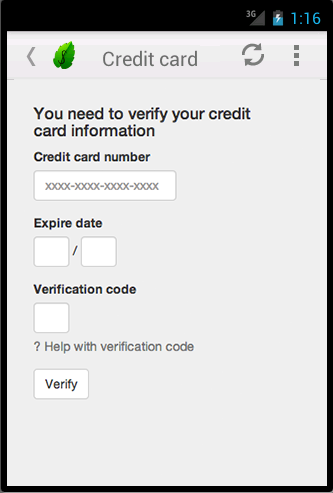
\includegraphics[width=1.8in]{./images/mint-example.png}
  \caption{Example of clickjacking attack on the Mint app.}
  \label{fig:mint}
\end{figure}

\textit{Mint} aggregates and presents to users detailed reports of all their incomes and expenses from different financial sources such as credit cards and bank accounts.
Our tool reported a \emph{entire screen} vulnerability in  Mint.
The UI integrity attack consists in showing to the user an arbitrary web page
inside the application visual context.
A clickjacking attack~\cite{android-clickjacking} scenario consists in presenting to the user a crafted web page resembling Mint's look and feel inside the application.
In the page, the user is asked to reinsert her credit card details complete
with verification code because of identity verification purposes. Reasonably, the user would act as asked, since they already inserted such information in the Mint system.
The loaded web page is now free to send the collected credit card information to any server. It is also important to point out that the URL of the currently visualized page is never presented to the user. An example of this attack can be seen in Figure~\ref{fig:mint}.

\textit{Poste Pay} manages the popular Poste Pay rechargeable debit card service, allowing users to recharge prepaid cell phones and any other Poste Pay card.
Our tool reported a \emph{alert screen} vulnerability in Poste Pay.
Since the content of an alert screen is completely specified by an attacker,
one could mimic traditional phishing attacks, prompting users to submit their information to a malicious website or email address. Another scenario could ask the user to make a small transfer to a specific credit card in order to, for example, extend the expiration date of the card.

\textit{Booking} is a hotel reservation system, allowing to browse hotels by geographical position, price and user rating and book them with the help of a credit card.
Our tool reported a \emph{entire screen} vulnerability in Booking.
The application allows attackers to fill arbitrary text in the ``Important Information'' screen.
An attack aimed to steal the reservation amount can be designed as follows: The user is informed of a (fake) server issue experienced by Booking itself, and told to proceed with a manual transaction to fake bank coordinates, or on an alternate (malicious) website.

\textit{GOSMS} is a popular SMS replacement client for Android for which
our tool reported a \emph{user input} vulnerability, which can be used to fill the SMS creation screen with arbitrary recipient and message body.
Exploiting this vulnerability, for instance, pre-populating the user inputs with a fake demand for
charity as SMS body one can set up an effective SMS fraud.
% We can just think at filling in the recipient field a crafted paid number used to collect money from user's prone credit.

% \textit{Mint}: is designed to aggregate and present to users detailed reports of all their incomes and expenses from different financial sources.
% The service produces the reports by periodically querying credit card and bank statements and by aggregating the transaction by time period and category.

% The tool reported that one of Mint's activities is vulnerable to an \emph{entire screen} UI integrity attack, which results in showing to the user an arbitrary web page inside the application visual context. An attacker may exploit this vulnerability to create sophisticated clickjacking attacks~\cite{android-clickjacking}. An attack scenario consists in presenting to the user a crafted web resembling the Mint look and feel inside the Mint application.
% In the page, the user is asked to reinsert her credit card details complete
% with verification code because of identity verification purposes. Reasonably, the user would act as asked, since they already inserted such information in the Mint system.
% The loaded web page is now free to send the collected credit card information to any server. It is also important to point out that the URL of the currently visualized page is never presented to the user. An example of this attack can be seen in Figure~\ref{fig:mint}.

% \textit{Poste Pay} is a financial application by the Italian postal service company offered to manage the popular Poste Pay rechargeable debit card service. In the application, the user can access cards statements, recharge prepaid cell phones or even recharge any other Poste Pay card by users card credit. Using our approach, we were able to design a scam attack simulation by prompting messages to the users (i.e. an \emph{alert screen} UI integrity attack). Since the content of the message is completely specified by an attacker, a scenario could mimic traditional phishing attacks, prompting users to submit their information to a malicious website or email address. Another scenario could ask the user to make a one dollar transfer to a specific credit card in order to, for example, extend the expiration date of the card.

% \textit{Booking} is the mobile application of the omonimous popular online hotel booking service, offering almost the same features as the website, such as
% making a reservation, browsing hotels by geographical position, price and user rating. The reservation service relies on a valid credit card. A reservation is successful if the card credit pre-authorization goes through.

% We found the application to be vulnerable, allowing attackers to fill arbitrary text in the ``Important Information'' screen in the Booking application (another instance of \emph{entire screen} vulnerability). An attack aimed to steal the reservation amount can be designed as follows. The user is informed of a (fake) server issue experienced by Booking itself, and told to proceed with a manual transaction to fake bank coordinates, or on an alternate (malicious) website.

% \textit{GOSMS} is a popular SMS replacement client for Android. It supports theming, private inbox, spam blocking and a large range of custom emoticons. Thanks to our analysis, we were able to generate a \emph{user input} attack, by populating the SMS creation screen with arbitrary recipient and message body. An attacker may exploit this vulnerability, for instance, by creating a SMS fraud, pre-populating the user inputs with a fake demand for charity as SMS body. Then, (s)he fills in the recipient field a crafted paid number used to collect money from user's credit.

% \subsection{Defensive Applications}
% Here we want to describe a particularly interesting sample we came across
% while performing the analysis. In this case, the
% string solver was unable to define sample input strings that could go through
% the paths to the vulnerable sink.

% In the GoChat application we noticed a recurrent parameter included in the Intents
% exchanged between application components, also in cases not marked as vulnerable
% from the analyzer. The string solver was unable to find a solution for such
% parameter because of a constraint that we were not completely able to specify.
% Before marking this case as pathological, we went back to manually inspect the
% application decompiled code. By reconstructing a whole communication example
% between two application components we ware able to understand the reason why the
% analyzer failed in its execution. This parameter represents an authorization
% code exchanged between the sender and the receiver of the Intent to guarantee
% message sender authenticity. The exchanged code is compared by the receiver to
% the content of a intra-component same-application shared variable. If there a
% match is not encountered the execution of the sender is immediately stopped. We
% can compare this approach to the one used in web application exchanging CSRF
% tokens. Of course because of the randomness in the parameter, no static analysis
% technique would be able to guess the valid token.

% This solution is very effective in practice, since guarantees complete
% protection to application resources possibly exposed to Intent attacks by
% completely blocking the normal execution flow. Unfortunately this solution is
% not generalizable to the case in which the receiver is intended to be accessed
% by selected application. Because of application sandboxing, two different
% application can not share (or partially share) memory parts.

% Instead, in Twitter, we found a server-based authorization mechanism. We found 5
% potential network vulnerabilities in the application. In this application the
% marked Intent messages are decorated with an user token. This token is included
% in the request sent to the server. Of course, the request succeeds only if the
% transmitted token is a valid one. Also in this case statically determining a
% valid token is impossible.

% Differently to the solution presented earlier, this approach, relying on an
% external (trusted) resource, the application server, can fulfill requests for
% other applications that have already obtained valid server credentials. These
% credentials usually are exchanged as consequence of an OAuth session.
% Credentials given to third party applications can, usually, easily be revoked by
% the user itself from the application's server.

\subsection{Other experimental results}

\begin{table*}[t]
\small
  \centering
  \begin{tabular}{|l|c|c|c|}
    \hline
    & Min & Max & Avg \\ \hline
    Per-application execution time & 2.4 min & 33.2 min & 12.3 min \\
    Per-application components & 3 & 31 & 24.5 \\
    Per-application vulnerable paths & 2 & 19 & 4.2 \\
    Per-path statements & 5 & 81 & 17.2 \\
    Per-path if-statements & 0 & 3 & 0.98 \\
    \hline
  \end{tabular}
  \caption{Other experimental setup}
  \label{table:other_experimental}
\end{table*}

In Table~\ref{table:other_experimental} we summarize several performance results, including information about analysis execution time, path lengths and components in the applications, and so on. As it can be noted, the execution time of our whole analysis depends on the number of components of an application. The per-application
execution time range is very wide, varying from a minimum of 2.4 minutes for 3 analyzed components to a maximum of 33.3 minutes spent to analyze an
application including 31 components, with an average of 12.3 minutes per application. The execution time is heavily dominated by the IFDS analysis which consists in 70-80\% of the overall execution time.

\todo{Second sentence in this paragraph is a little bit unclear}
We discovered 92 paths leading to a sink out of 537 analyzed with an average of 4.2 vulnerable paths per application. For each vulnerable path the analyzer collected an average number of 17.2 statements, with an average number of 5.8 statements including API calls. We approximated 31.2\% of the supported API methods by not giving precise formulations due to Kaluza limitations, as described in Section \ref{section:kaluzaTranslation}. We found this not to be a limitation to our approach for two reasons: this apparently large number of approximations were performed, in practice, over the 7.7\% of the total number of translated statements including library calls, meaning that approximated transformations are, in general, infrequent.
Second, it is worth noting that within the analyzed paths, very few include validation checks over the data in input. In particular, our tool found at most 3 checks in those paths, usually checks on null values. In short validation checks involving Intent payloads are performed in the 23\% of the vulnerable paths.

\subsection{Discussion of Results and Recommendations}

From our results, it is clear that only a few applications properly implement validation of data received from Intent messages. Most applications perform only basic checks on Intent payloads parts, such as null-checks, performed only to protect against malformed Intents payload tuples. Such checks are not strict enough to defend application resources against more sophisticated Intent spoofing attacks as the ones we considered in this work.

In order to verify the intents' origins, currently developers may need to implement custom authentication mechanisms, given the absence of a system-provided intent origin verification feature. A recommended solution consists in exchanging keys between intent sender and receiver, and requiring signatures to be exchanged within intents as a mean of authentication. This solution is very similar to the one used in web application exchanging CSRF tokens, and it is very effective in practice, since it guarantees complete protection to application components possibly exposed to Intent attacks. However, it requires communication of key material among applications before normal communications can start.
% this solution is
% not generalizable to the case in which the receiver is intended to be accessed by selected application. Because of application sandboxing, two different application can not share (or partially share) memory parts.

An OS-level enhancement to offer to final users a set of features
in the Intent API to reliably retrieve an intent's origin or sign intent's data would also help mitigate this risk. A work that proposes something similar can be found in~\cite{quire2011}.
% Offering such features means in practice to insert in the environment an additional trusted entity
% in charge of generating and validating communication signatures. An encrypted communication channel with a verified remote server may also help in solving this problem, even though it would not be practical.

Most importantly, developers should always include strong data validation checks, even when dealing with intents, and should follow all the guidelines to securely implement intent communications by not exposing their application components unnecessarily.


% !TEX root =  ../main.tex
\section{Related Work}
\label{sec:related}

Android ICC security has received an increasing interest in the past years. 
The current state of the art is presented in \cite{Epicc}. This work aims to provide a precise specification of applications ICC interconnections by using IFDS analysis to determine communication entry and exit points and determine security breaches. Despite some common points in the techniques, our work is focused on the paths inside a single application rather than analyzing a network of intercommunicating applications. In addition, we characterize vulnerabilities and provide exploit proofs. 

In \cite{chin2011analyzing}, the authors analyze the inter-application message passing system and identify risks of intent-spoofing, such as broadcast eavesdropping and denial of service. Their work is however focused on developer practices that allow intents to be sent by malicious applications and received by victim applications. Our work goes more in-depth and focuses on how the attackers can use intent-spoofing and leverage insufficient intent data validation checks inside applications to carry out additional attacks. Also, our work goes in the direction of automatic detection and exploitation of the vulnerabilities.

In FlowDroid, the authors present an IFDS-based taint analysis to derive information flow inside Android applications and detect malicious data leakages~\cite{flowdroid}. Conversely, in our work, IFDS-based taint analysis is used only as a first step towards symbolic execution of an application component with the goal of finding vulnerable paths inside an application.

A work related to defenses against intent spoofing is~\cite{quire2011}. Quire is a lightweight framework to enhance Android IPC mechanism by adding message provenance. The implementation relies on a signature scheme that allows message recipient validation before delivering. The class of attacks they want to prevent is closely related to the ours: \emph{confused deputy attacks}. Their approach needs to modify the Android OS in order to guarantee the described security features, our approach aims to obtain a similar result by preventing behaviors that can potentially introduce vulnerabilities in applications.

Other related studies includes different techniques for statically testing 
security of Android applications: Schmidt \emph{et al.}~\cite{schmidt2009static} used static analysis to extract a 
list of function calls from which they can perform data analysis for malware 
detection. Mirzaei \emph{et al.}~\cite{mirzaei2012testing} applied symbolic execution techniques in order to generate test cases and thus differs significantly from our work. ScanDal~\cite{kim2012scandal} is a static analyzer that implements a formal approach to automatically detect private data leaks in Android applications rather than detect active attacks as in our work. AppIntent~\cite{AppIntent} uses symbolic execution to detect if dataflows from application GUI elements are not intended by the user and differs from our approach for detecting vulnerabilities and providing proofs for them. 

\todo{W3 Discussion about Dowser}

% A very broad area of research relates with the development of various techniques for malware analysis: from their classification~\cite{zhou2012dissecting}, 
% behavior reconstruction~\cite{reina2013system} and deep analysis~\cite{yan2012droidscope} to their detection~\cite{burguera2011crowdroid, grace2012riskranker}. However, none of these works deals with legitimate application analysis and detection of insufficient validation checks among applications.



% !TEX root =  ../main.tex
\section{Conclusions}
\label{sec:concl}

In this paper, we describe an automated analysis framework to study validation checks over the data received via Intent messages in Android applications. Our method for automatically detecting these vulnerabilities relies on static taint analysis and symbolic execution, using the IFDS framework. Furthermore, we use a solver to automatically generate a  proof-of-concept attacker app that validate the vulnerabilities. We evaluate our approach on 64 popular applications downloaded from the Google Play Store, finding 29 potential vulnerabilities, and automatically exploiting (and thus confirming) 26 of these. Our results confirm that a large percentage of commonly-used applications do not implement appropriate security safeguards for Intent communications.

\bibliographystyle{IEEEtran}
\bibliography{bibliography}

\end{document}
